\subsection{Gabor Wavelets in Variational Autoencoders}\label{subsec:results_visual_features_in_variational_autoencoders}
Simple and cells in \ac{V1} show the strongest excitation for Gabor wavelets (see Section~\ref{subsubseq:simple_complex_cells}).
As discussed earlier, the optimal stimulus for a convolutional kernel resembling a Gabor wavelet, is a Gabor wavelet itself (see Section~\ref{subsubsec:cnn_model_visual_system}).
Therefore, the emergence of Gabor-like filters is considered evidence for a model's biological plausibility~\citep{berkes2005slow}.
\citet{krizhevsky2012imagenet} found that AlexNet learns Gabor-like features in the first layer.
It was later found that supervised \acp{CNN} like AlexNet explain \ac{IT} activity~\citep{khaligh2014deep}.

Therefore, emergence of Gabor wavelets in \acp{VAE} would be evidence for their suitability as a model of the visual system.
Potentially, they would even indicate that higher layers explain activity of higher regions in the visual cortex.
Therefore, the following experiment was conducted.

Since it is known that AlexNet learns Gabor wavelets in lower-level filters, a \ac{VAE} network with a similar architecture (AlexNet-\ac{VAE}, see Section~\ref{subsubsec:alexnet_vae}) was designed.
The hypothesis is that if \acp{VAE} can learn Gabor wavelets, this model should show them because it is very similar to the supervised model for which they are learned.
First, it was verified that the supervised network (AlexNet Classifier, see Section~\ref{subsubsec:alexnet_classifier}) actually learns Gabor wavelets.
The network was trained for ten epochs, the top-1 training accuracy at this time was at 0.85.

\begin{figure}
    \centering
    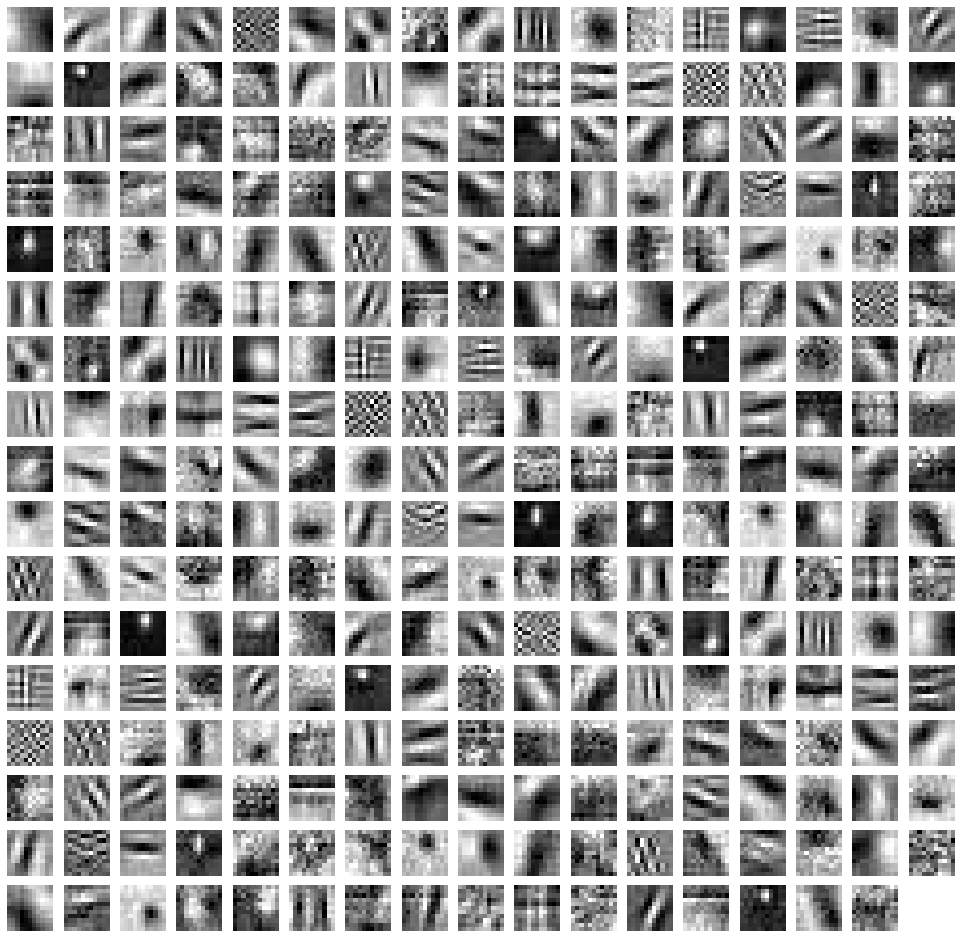
\includegraphics[width=0.9\textwidth]{images/alexnet_classification_l1_kernels.png}
    \caption[Image classification - Layer 1 Kernels]{Convolutional Kernels in the first layer of the image classification network. The filters are shown in their original size (11x11).}
    \label{fig:classification_layer1_kernels}
\end{figure}

\begin{figure}
    \centering
    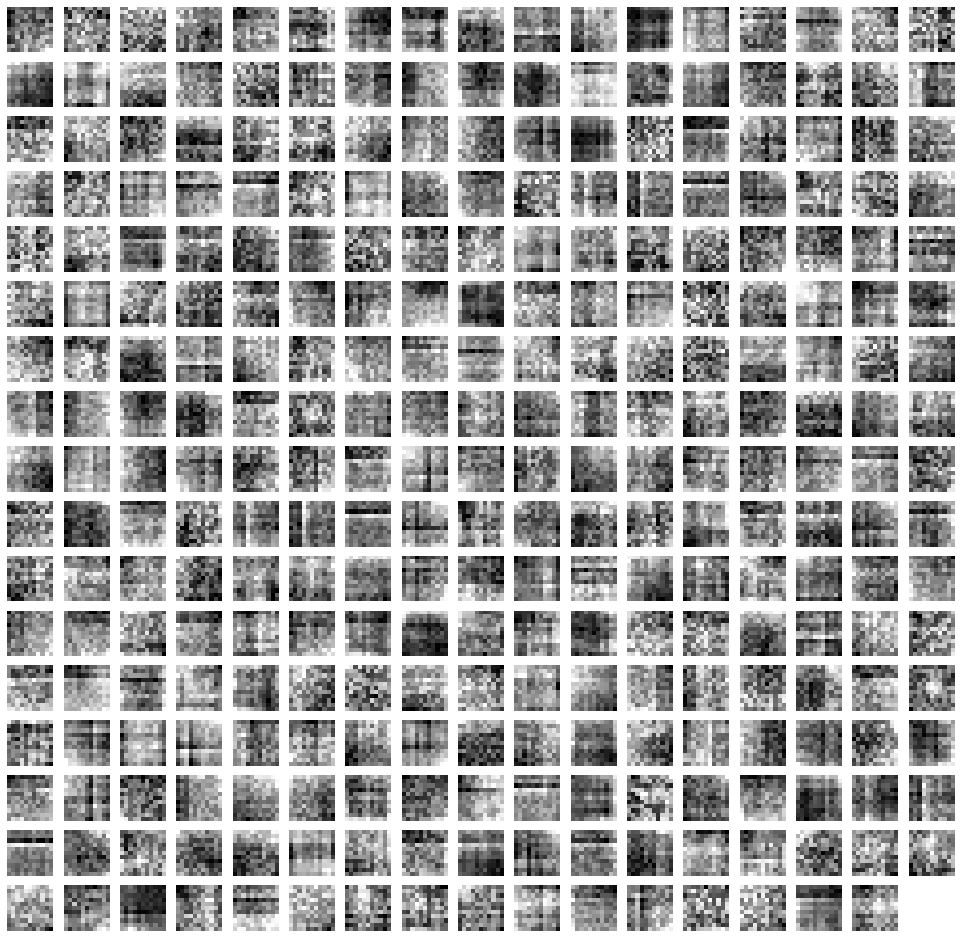
\includegraphics[width=0.9\textwidth]{images/alexnet_vae_l1_kernels.png}
    \caption[VAE - Layer 1 Kernels]{Convolutional Kernels in the first layer of the AlexNet \ac{VAE} network. The filters are shown in their original size (11x11).}
    \label{fig:vae_layer1_kernels}
\end{figure}

Figure~\ref{fig:classification_layer1_kernels} shows all 288 ($96 \cdot 3$) convolutional kernels of AlexNet Classifier\footnote{See Section~\ref{subsubsec:alexnet_classifier}.}.
In many kernels, Gabor wavelet-like filters emerge.

However, the same effect cannot be observed in the kernels AlexNet-\ac{VAE}\footnote{See Section~\ref{subsubsec:alexnet_vae}.}.
Figure~\ref{fig:vae_layer1_kernels} shows the kernels of the first layer in AlexNet-\ac{VAE}.
Moreover, no Gabor wavelets emerged in any of the models\footnote{All models described in Section~\ref{subsec:models} apart from AlexNet Classifier.} or for any of the datasets.

It is therefore concluded that a simple feed-forward \ac{VAE} or \ac{VLAE} trained to generate dense representations of static images probably cannot learn Gabor-wavelets.
This does not imply that \acp{VAE} or \acp{VLAE} do not explain cortical activity (this is discussed in Section~\ref{subsec:representational-dissimilarity-matrices}).
Furthermore, variations of the \ac{VAE}-design are proposed that could lead to a more biologically plausible model (see Sections~\ref{subsec:feedback-connections-of-the-lateral-geniculate-nucleus} and \ref{subsec:sequential-data}).

% TODO: show generations and reconstructions of AlexNet VAE

\subsection{Sparseness in Generative Models}\label{subsec:effective-network-capacity}
One hyperparameter to choose in the different models is the number of feature maps of different layers.
During the implementation, it was observed that some feature maps show little activity compared to others.
As the number of features maps is a model hyperparameter, it was investigated by how much the number of feature maps can be reduced without increasing the network loss.

Furthermore, the question arose whether sparseness in \acp{VLAE} is related to sparseness in the primary visual cortex (see Section~\ref{subsubsec:sparse_representations}).
Even though \acp{VAE} and \acp{VLAE} do not learn Gabor wavelets in lower layers, they could superpose sparse set of different basis functions to represent their input, similar to \citet{Olshausen1996}.
If they do, this would be evidence for the relatedness of \acp{VLAE} to the biological example.

The following experiment was conducted to examine if \acp{VLAE} employ sparseness or if the model has only too much capacity.
The feature map activity of \ac{VLAE}s on \textsc{Mnist} with input size $28\times 28$ and different numbers of feature maps and nodes in fully connected layers was measured.
By gradually decreasing the network capacity, the evolvement of sparseness was analyzed.
In total, three models (\textsc{Mnist}-\ac{VLAE}-factor-1, \textsc{Mnist}-\ac{VLAE}-factor-2, and \textsc{Mnist}-\ac{VLAE}-factor-3, see Section~\ref{subsubsec:vlae_models}) were trained.
Batch normalization was disabled for this experiment, because it re-scales the feature map activity.

\begin{figure}
    \centering
    \begin{subfigure}{.95\textwidth}
        \centering
        % include first image
        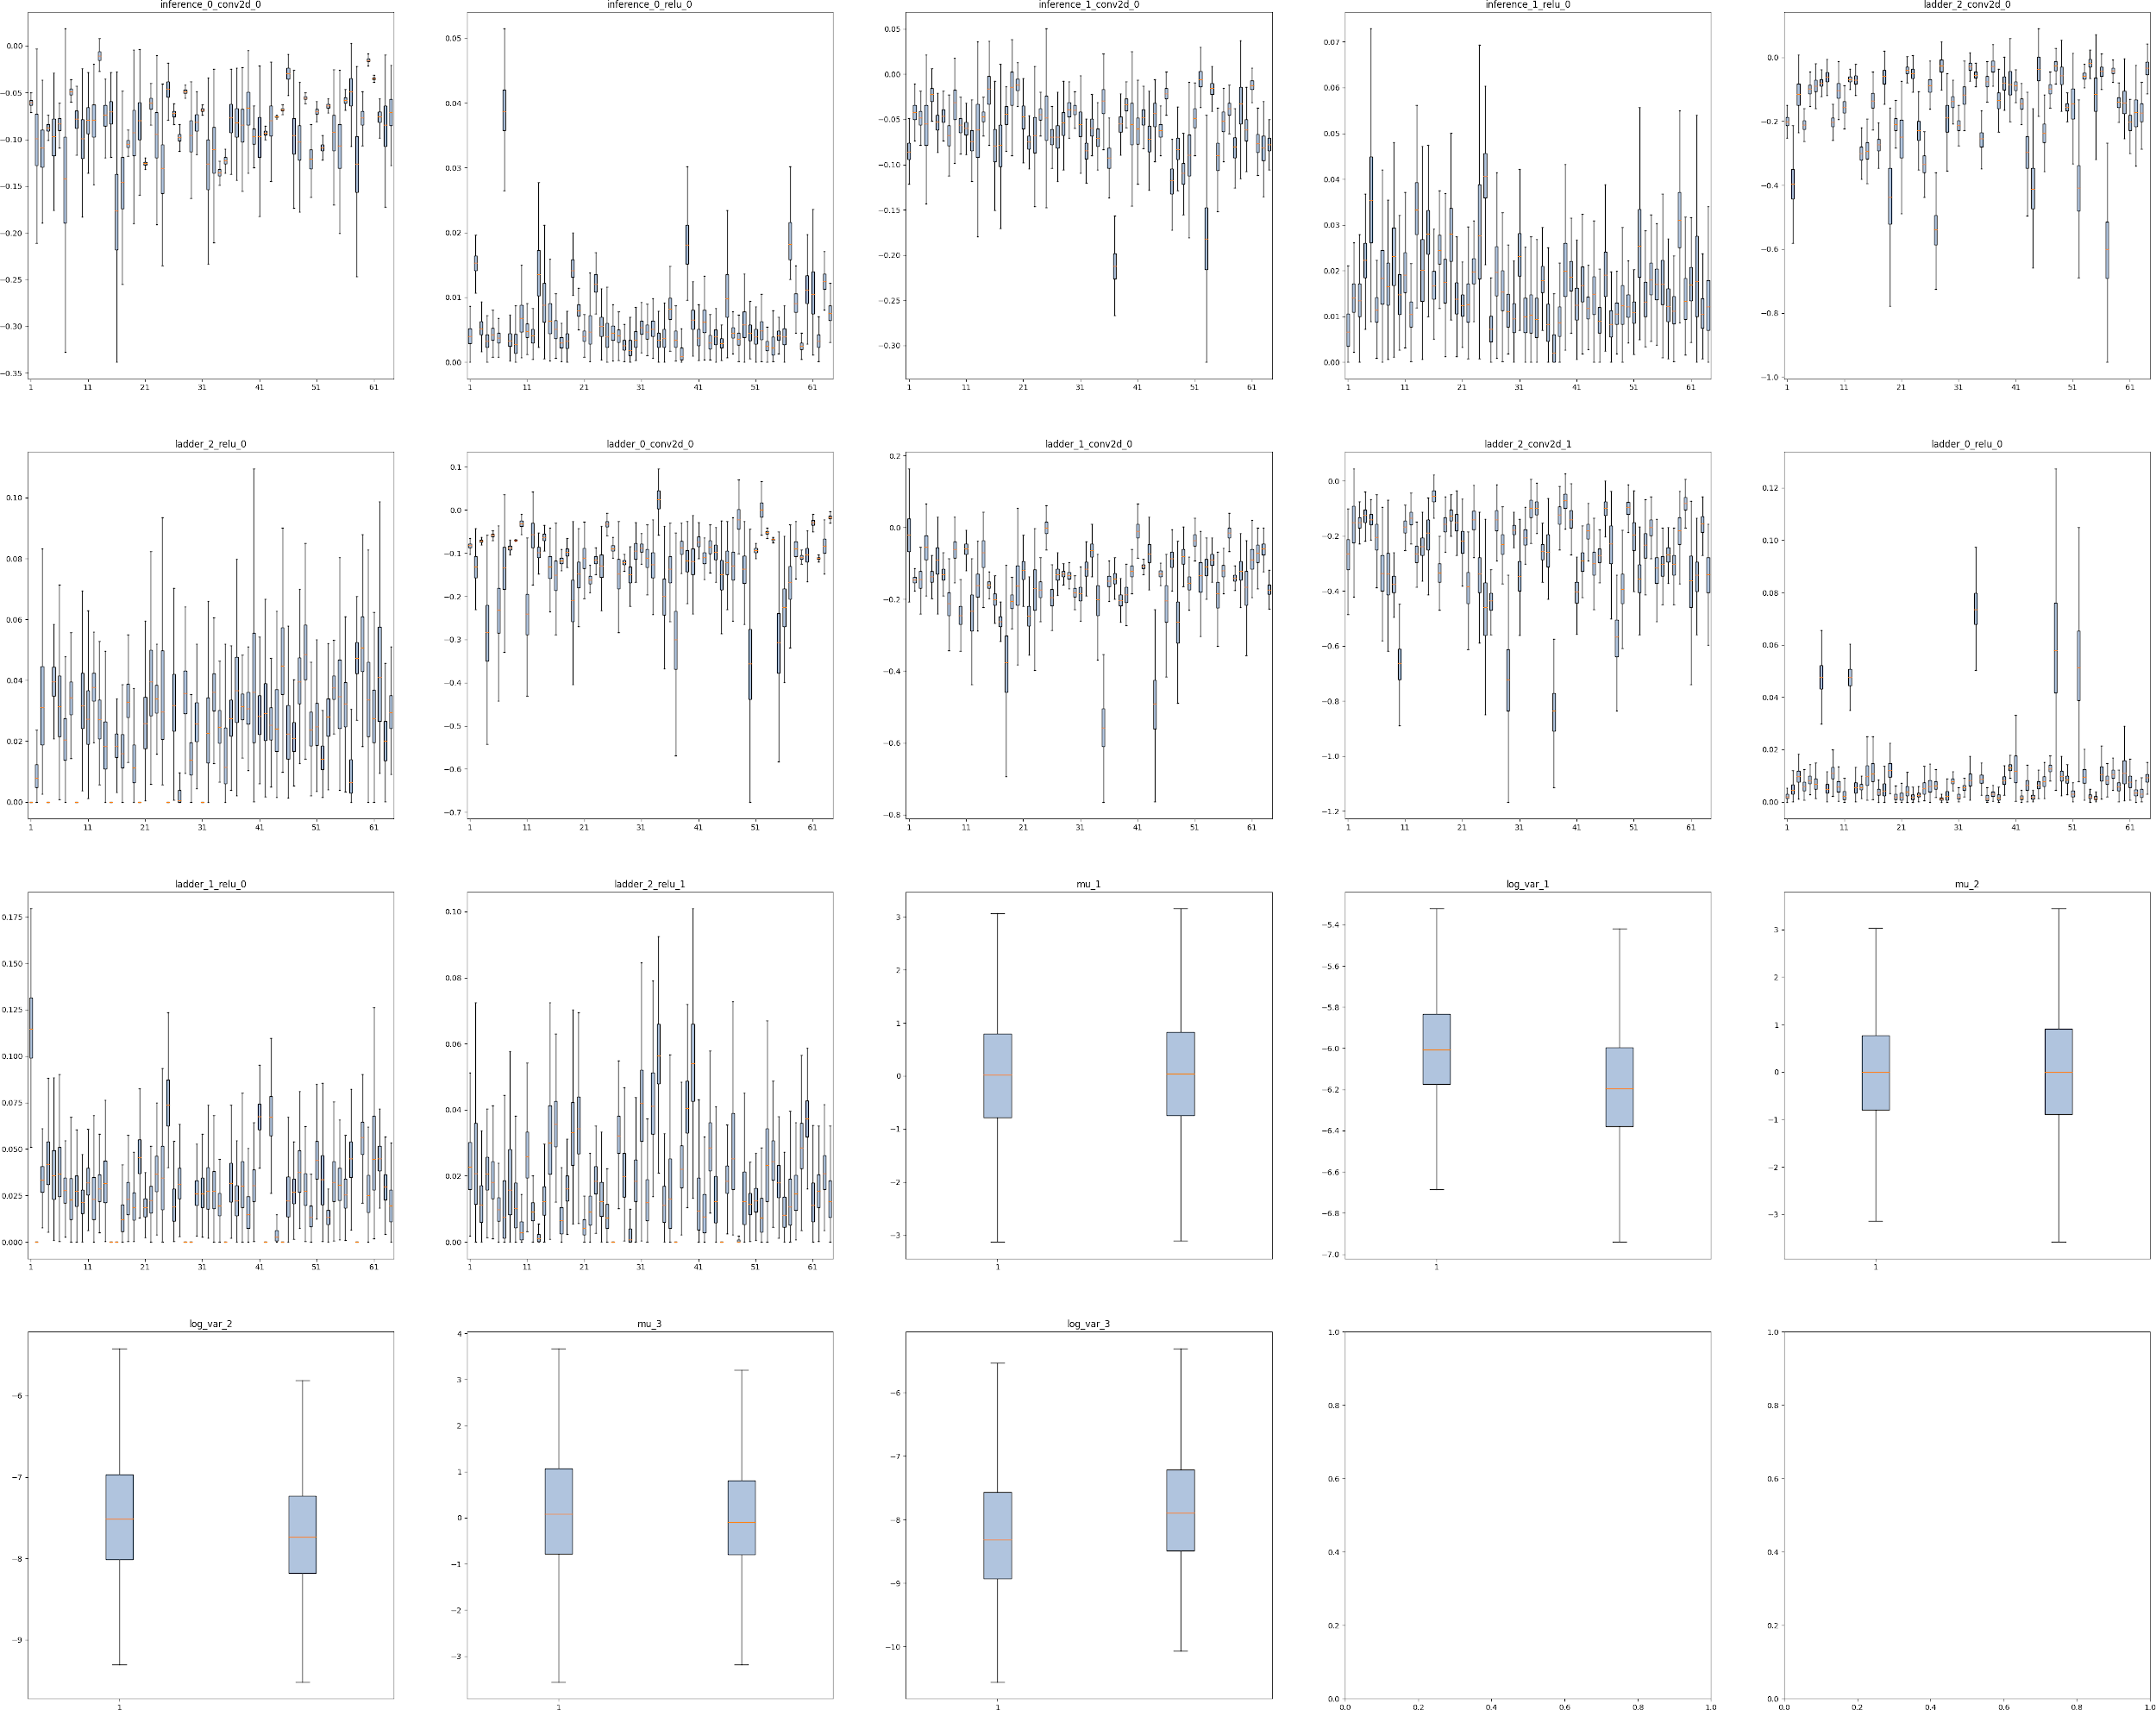
\includegraphics[width=\textwidth]{images/sparseness/encoder_fm1_fms.png}
        \caption{Feature map activities - large model}
    \end{subfigure}
\end{figure}
\begin{figure}
    \ContinuedFloat
    \centering
    \begin{subfigure}{.95\textwidth}
        \centering
        % include second image
        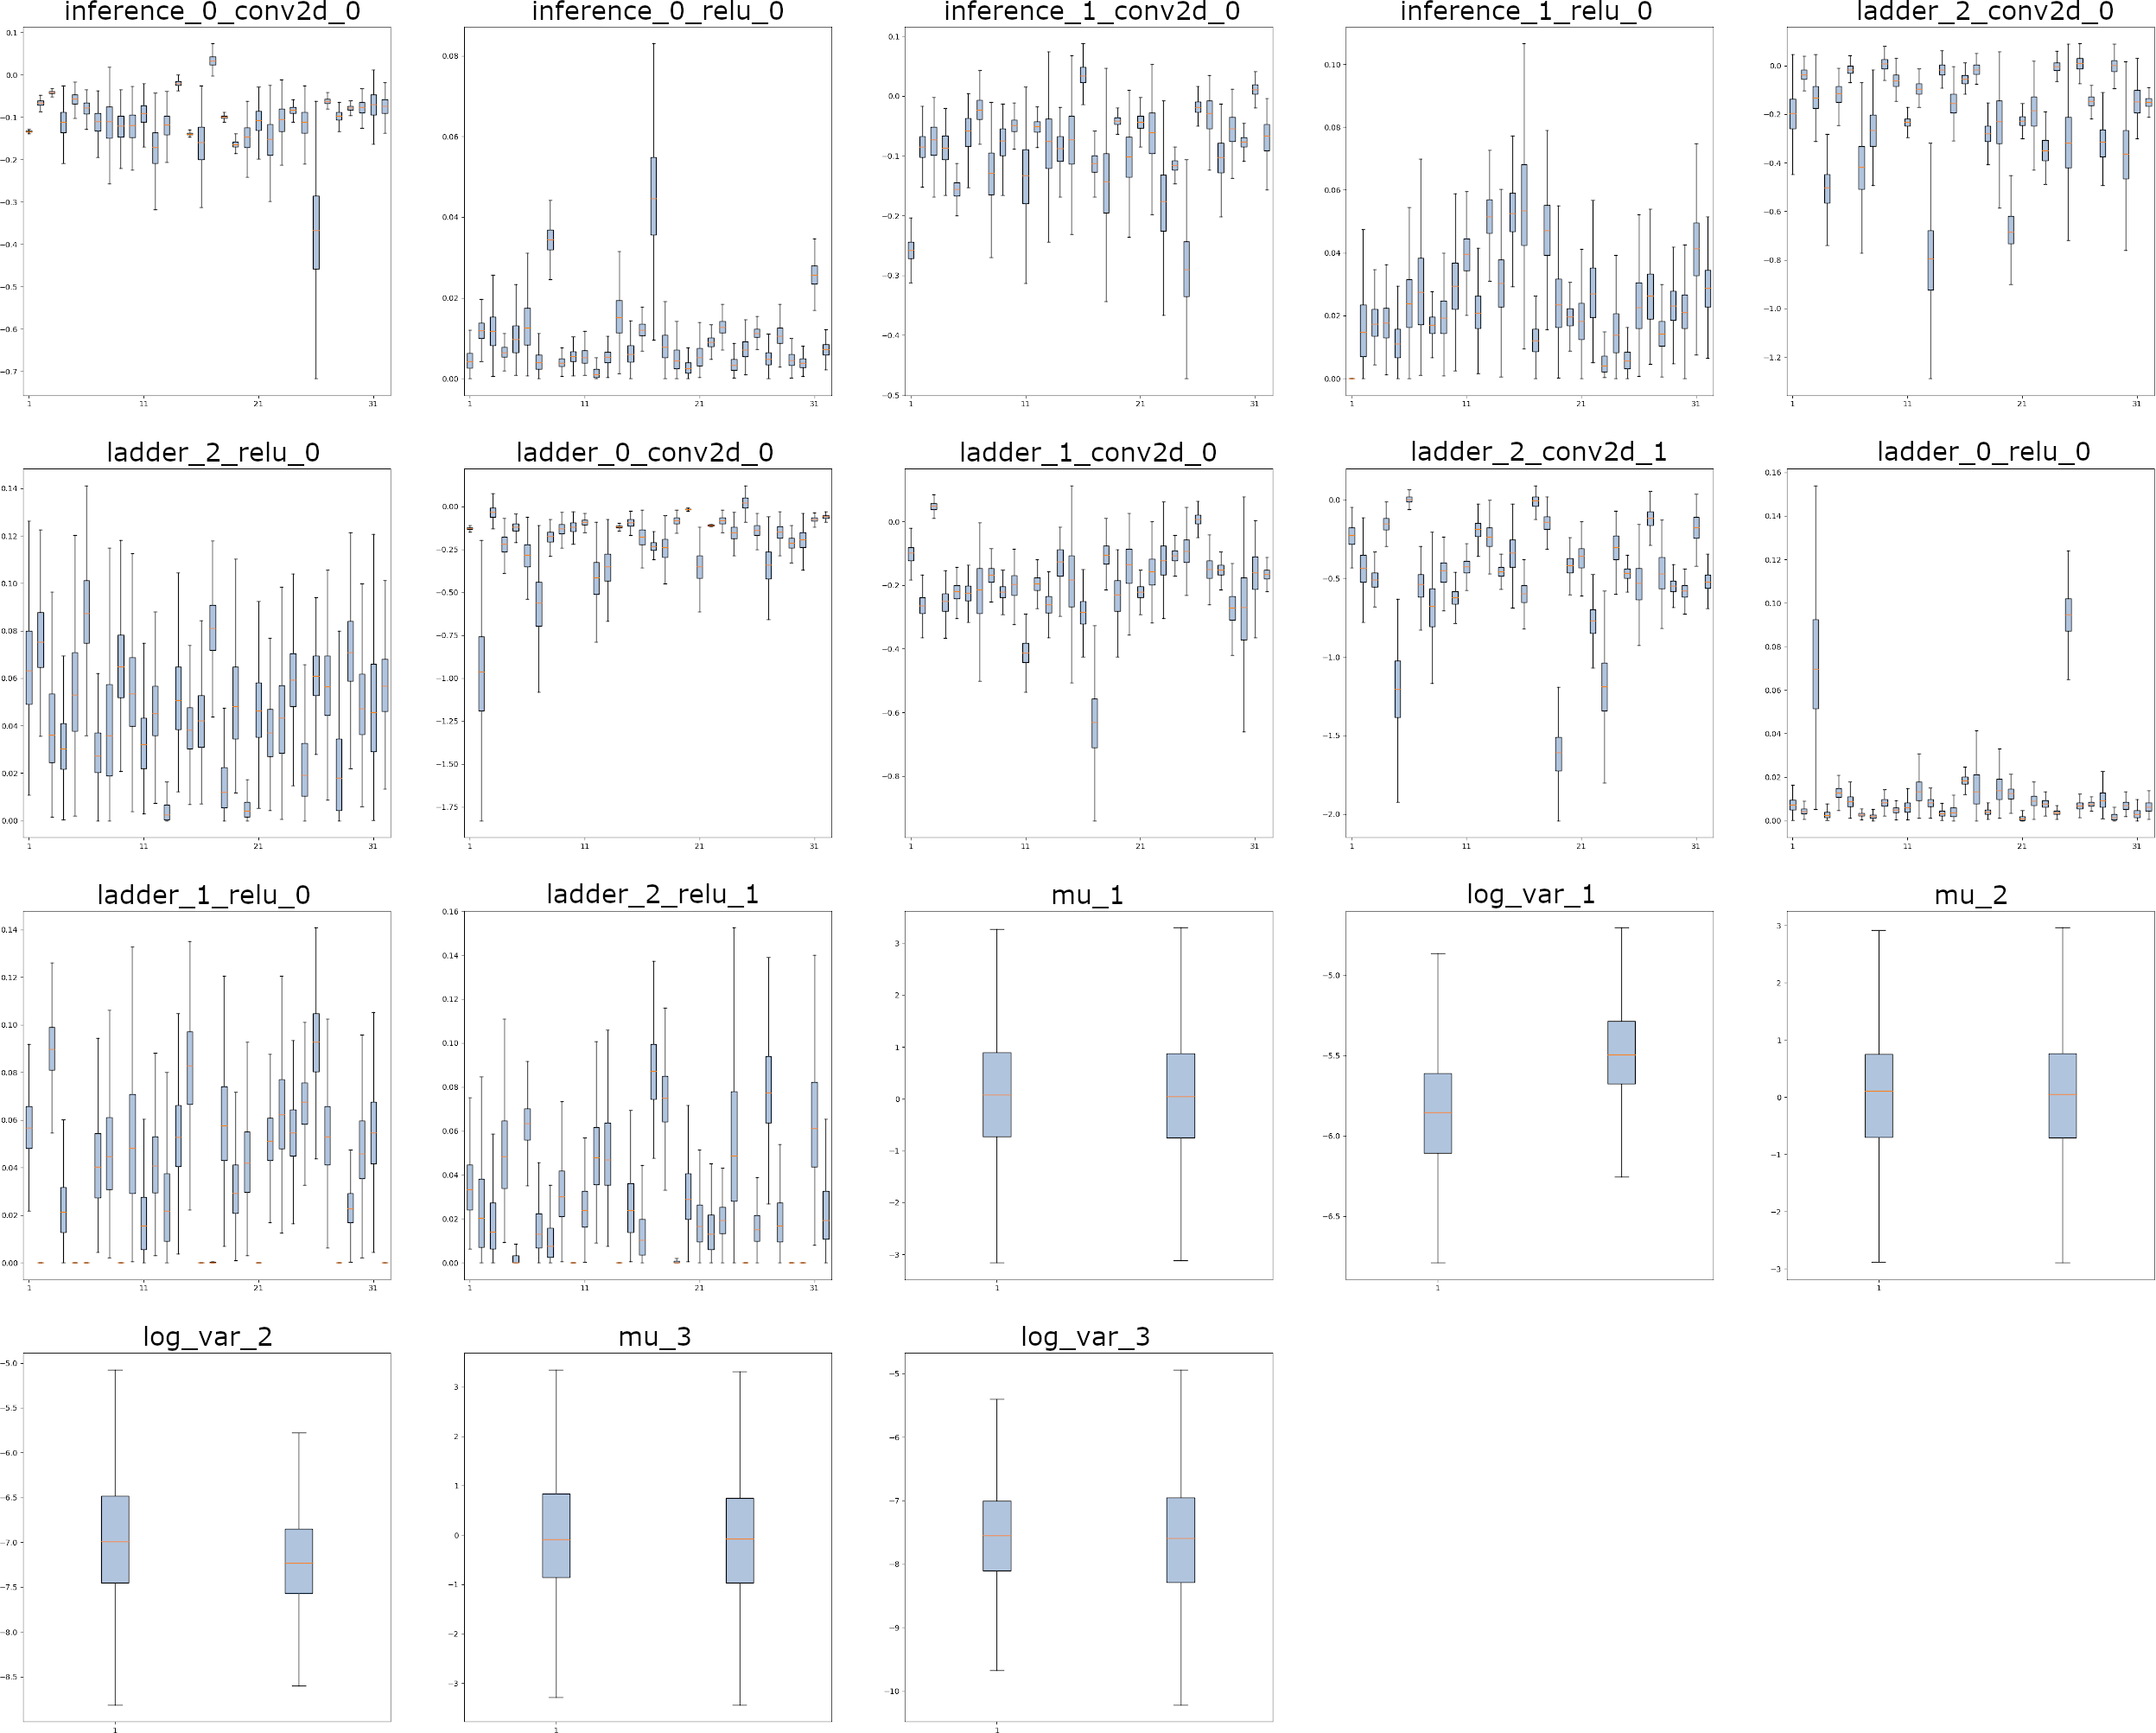
\includegraphics[width=\textwidth]{images/sparseness/encoder_fm2_fms.png}
        \caption{Feature map activities - medium model}
    \end{subfigure}
\end{figure}
\begin{figure}
    \ContinuedFloat
    \centering
    \begin{subfigure}{.95\textwidth}
        \centering
        % include second image
        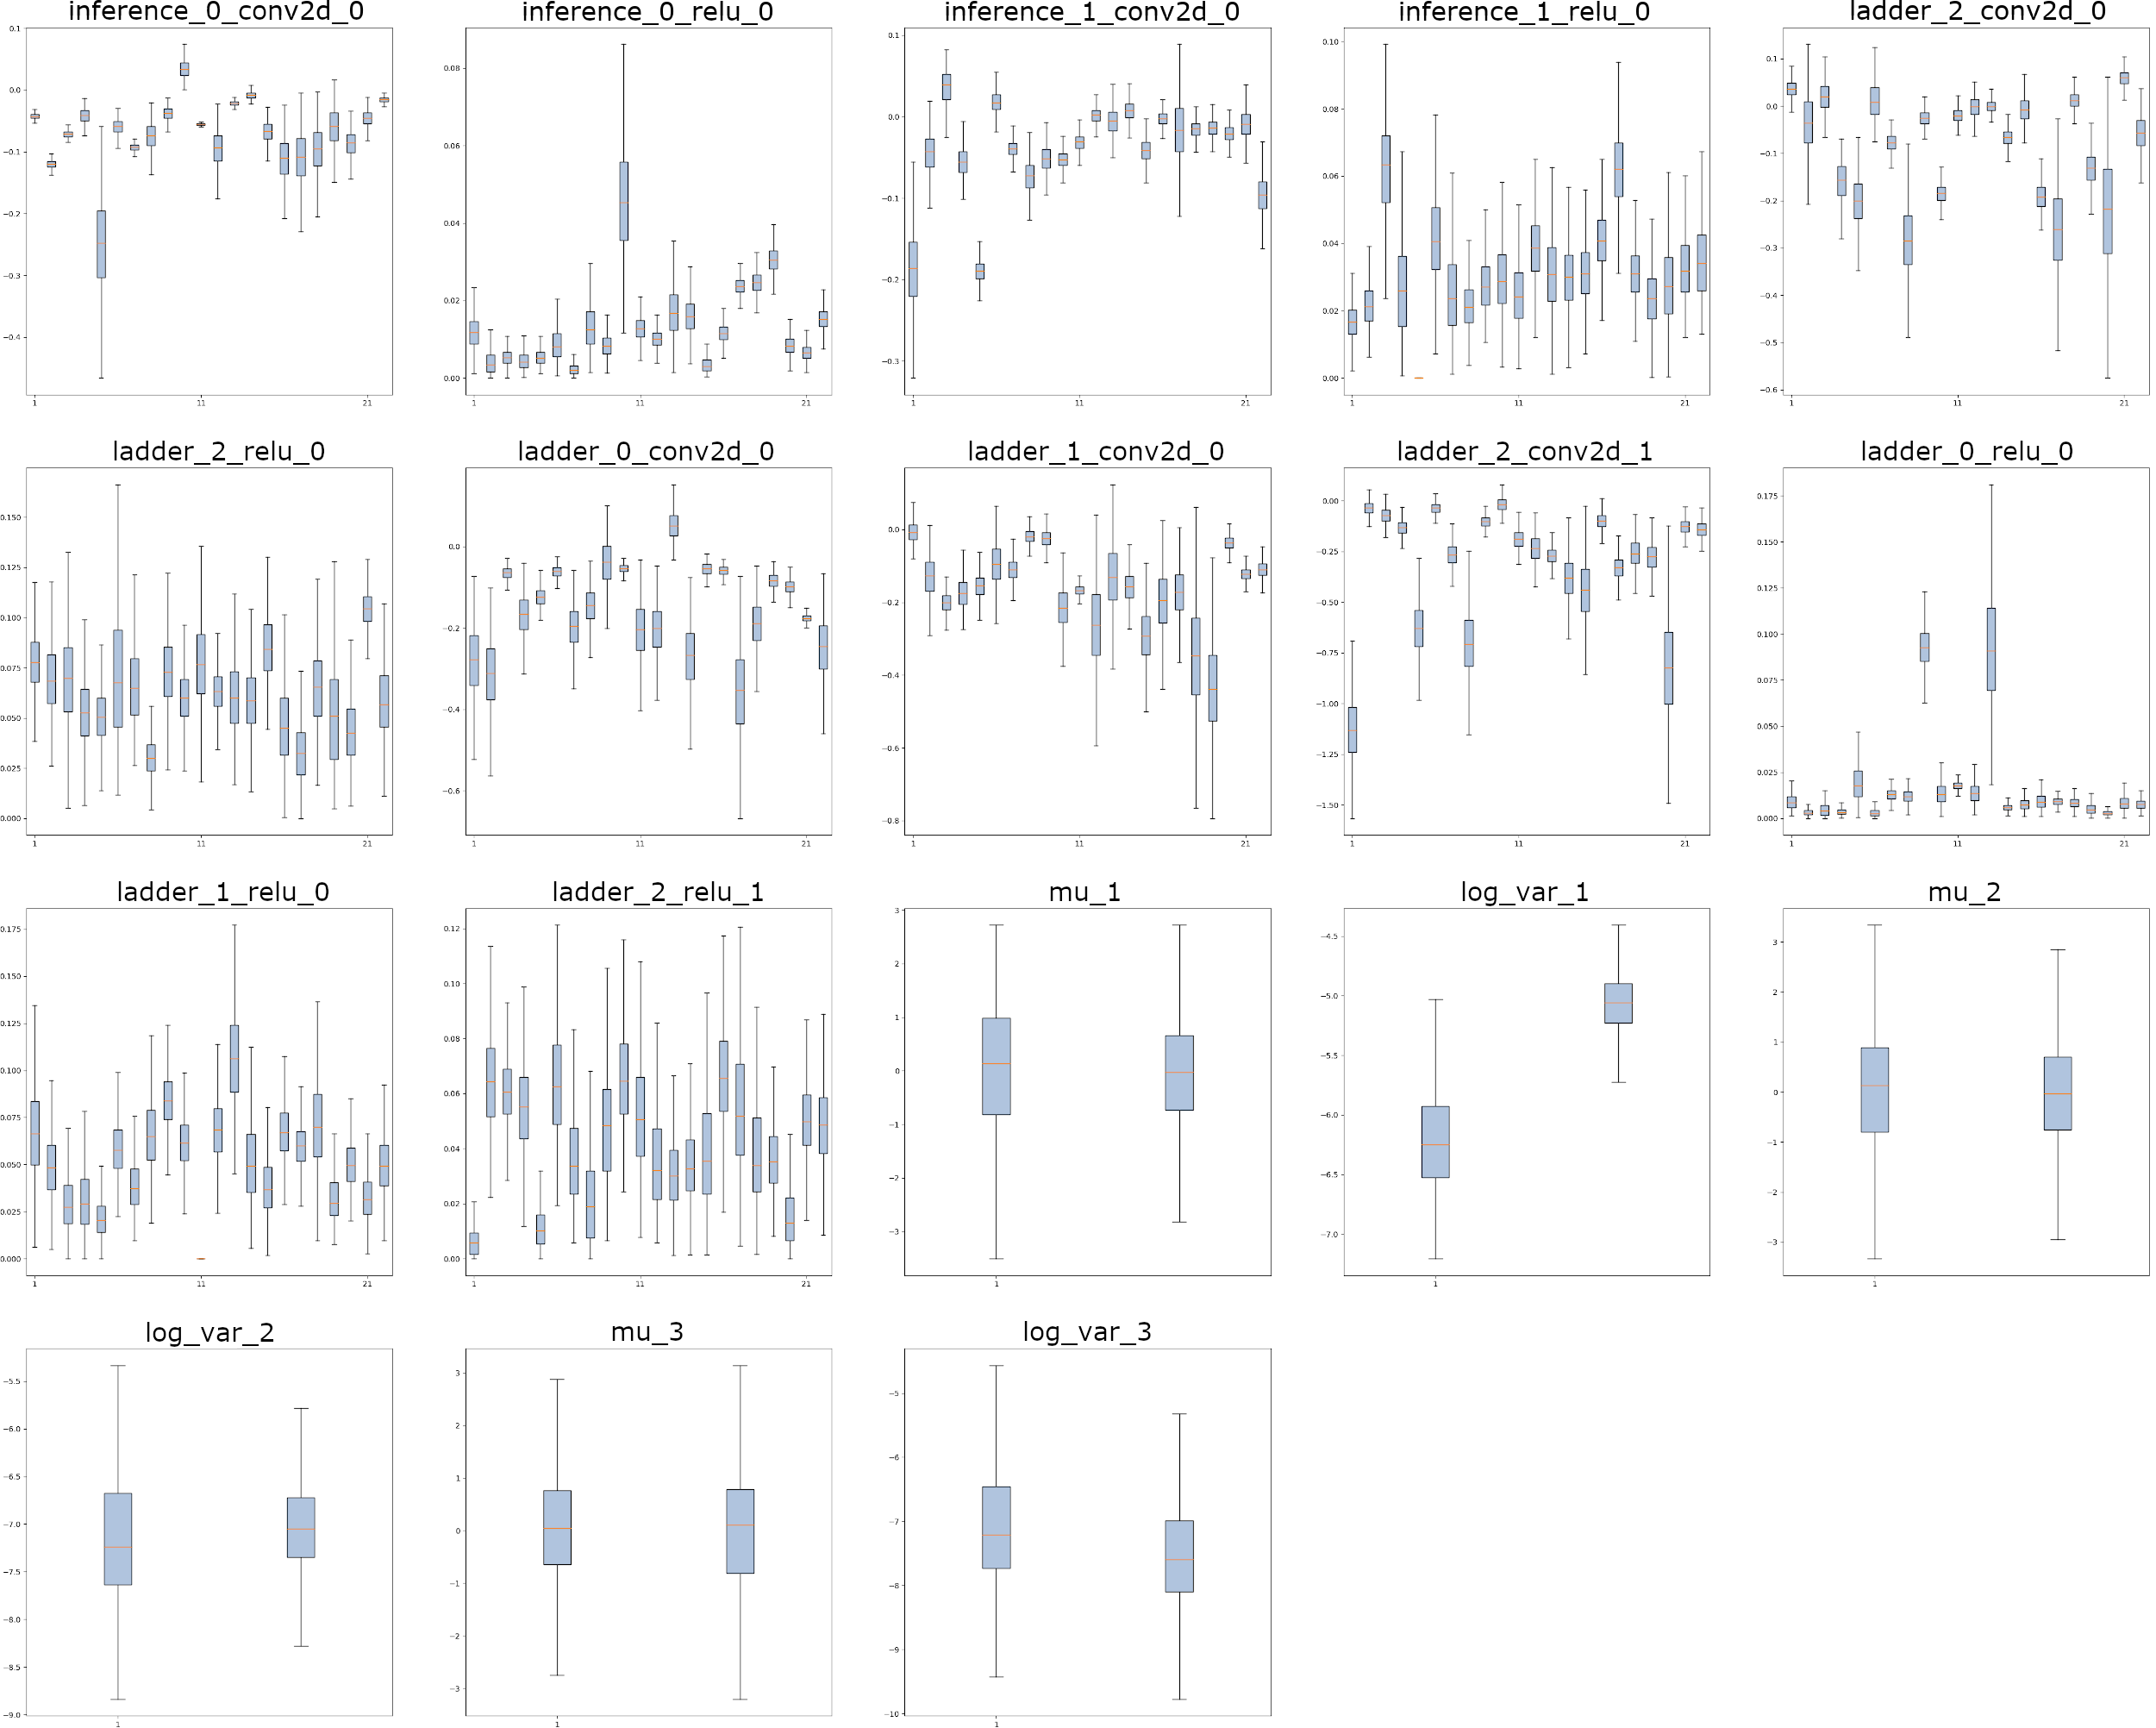
\includegraphics[width=\textwidth]{images/sparseness/encoder_fm3_fms.png}
        \caption{Feature map activities - small model}
    \end{subfigure}
    \caption{Feature map activities for the different models}
    \label{fig:fm_activities_sparseness}
\end{figure}
\begin{figure}
    \centering
    \begin{subfigure}{.45\textwidth}
        \centering
        % include first image
        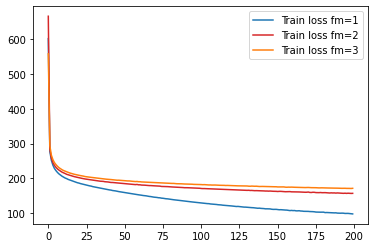
\includegraphics[width=\textwidth]{images/sparseness/sparseness_train_loss.png}
        \caption{Training loss}
    \end{subfigure}
    \hfill
    \begin{subfigure}{.45\textwidth}
        \centering
        % include second image
        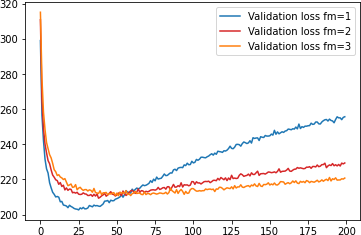
\includegraphics[width=\textwidth]{images/sparseness/sparseness_validation_loss.png}
        \caption{Validation loss}
    \end{subfigure}
    \caption[Sparse Models - Loss Curves]{Loss curves of models with different numbers of feature maps (see Section~\ref{subsubsec:vae_models}). $fm$ is the reduction factor of the feature maps; $fm=1$, therefore, is the original model, $fm=2$ the model with half the number of feature maps, and $fm=3$ the model with one third of the feature maps.}
    \label{fig:learning_curves_sparseness}
\end{figure}

Figure~\ref{fig:learning_curves_sparseness} shows the training and validation losses for the models.
Firstly, increasing the number of feature maps increases convergence speed.
Even though \textsc{Mnist}-\ac{VLAE}-factor-1 is trained with a slightly lower learning rate, it converges faster than \textsc{Mnist}-\ac{VLAE}-factor-2 and \textsc{Mnist}-\ac{VLAE}-factor-3.
It also achieves the lowest validation loss among the three models and achieves the minimum validation loss faster than the other models; it is minimal after 26 epochs for \textsc{Mnist}-\ac{VLAE}-factor-1, 39 epochs for \textsc{Mnist}-\ac{VLAE}-factor-2, and 52 epochs for \textsc{Mnist}-\ac{VLAE}-factor-3.
After achieving the minimum validation loss, however, all models overfit.
\textsc{Mnist}-\ac{VLAE}-factor-1 overfits stronger than \textsc{Mnist}-\ac{VLAE}-factor-2 or \textsc{Mnist}-\ac{VLAE}-factor-3, leading to the highest validation loss after 200 epochs.

Figure~\ref{fig:fm_activities_sparseness} shows the activities of the feature maps in the different models.
Each line in a subplot is a boxplot and each subfigure the output of either a convolutional, activation, or fully connected layer.
Most prominently, the inner activations are sparse after convolutions.
The activations often increase the level of sparsity since the ReLU activation functions map negative values to zero.
Sparsity is apparent in almost all feature maps of all models.

\paragraph{Sparseness in \acp{VLAE} vs. Sparse Representations}
In the brain, the overlap of active neurons is small, i.e., different neurons are active for different stimuli (see Section~\ref{subsubsec:sparse_representations} and \citet{yoshida2020natural}).
Contrarily, the \acp{VLAE} show high activity mostly in the same feature maps regardless of the input.

The \ac{VLAE} uses sparseness mostly regardless of the model capacity, which can be explained by the Lottery Ticket Hypothesis~\citep{frankle2018lottery}.
The Lottery Ticket Hypothesis states that, in general, it is highly unlikely that re-training a pruned network from scratch will result in the same weight configuration of the subnetwork in the initial model.
In the three models (\textsc{Mnist}-\ac{VLAE}-factor-1, \textsc{Mnist}-\ac{VLAE}-factor-2, and \textsc{Mnist}-\ac{VLAE}-factor-3), there seems to be a sub-network that accounts for the activity in the model.
Regardless of the reduction factor, there always remains an active sub-network for all three models.

Therefore, the sparseness in \acp{VLAE} does not seem to be related to sparse representations in the brain.

\subsection{Latent Space Entanglement and Categorical Factors of Variation}\label{subsec:latent-space-entanglement-and-categorical-factors-of-variation}

As discussed in Section~\ref{subsec:feature-disentanglement} and Section~\ref{subsubsec:representation_learning} ($\beta$-\ac{VAE}), in practice, there is a trade-off between reconstruction quality and prior-posterior matching.
Again, the $\beta$-\ac{VAE} loss function is defined as
\begin{align}
    \mathbb{E}_{q_{\phi}(\bm{z} | \bm{x})}\left[\log p_{\theta}(\bm{x} | \bm{z})\right]-\beta \kldiv{q_{\phi}(\bm{z} | \bm{x})}{p(\bm{z})}. \label{eq:beta-vae-2}
\end{align}
Increasing the weight of the reconstruction term in the \ac{VAE} training objective (smaller $\beta$ in Equation~\ref{eq:beta-vae-2}\footnote{The $\beta$ in $\beta$-\ac{VAE} is the \ac{KL}-term weight. Therefore, decreasing $\beta$ analog to increasing the reconstruction term weight.}) leads to reconstructions more similar to the training samples.
The posterior distribution, however, matches the prior distribution less precisely.
Contrarily, increasing $\beta$ in Equation~\ref{eq:beta-vae-2} leads to a posterior closer to the prior distribution at the expense of reconstruction quality.
Moreover, \citet{higgins2017beta} claim that increasing $\beta$ leads to a better latent space disentanglement, i.e., each dimension in the latent space is uniquely correlated with a single factor of variation.

As discussed in Section~\ref{subsec:feature-disentanglement}, the quality of feature space disentanglement can be assessed by measuring how fast reconstructions change as the latent space is traversed.
Nevertheless, a disentangled feature space should be problematic for datasets with categorical factors of variation, such as dSprites, where features change fast by definition.
Even though CelebA has binary labels as well (e.g., \say{brown hair}), there still is enough variation within hair colors to allow a smooth translation between hair colors~\citep{higgins2017beta}.
For dSprites, there are only three distinct shapes (\say{square}, \say{ellipse}, and \say{heart}).
To achieve a good reconstruction quality on these shapes, the model would have to place them in separate areas of the latent space, violating both feature space disentanglement and a Gaussian posterior.

To analyze how \acp{VAE} behave for categorical factors of variation, a \ac{VAE} with input size $64\times 64$ (the size of dSprites images) and a ten-dimensional latent space was trained on dsprites with different reconstruction term weights: 10,000, 7,500, 6,250, 5,000, and 3,750 (see Section~\ref{subsubsec:vae_models})\footnote{It was first empirically validated that a reconstruction term weight of 10,000 leads to good reconstruction. The other values were chosen by reducing the reconstruction loss term by 1,250 for each model with a larger initial difference (10,000 vs. 7,500).}.

\begin{figure}
    \centering
    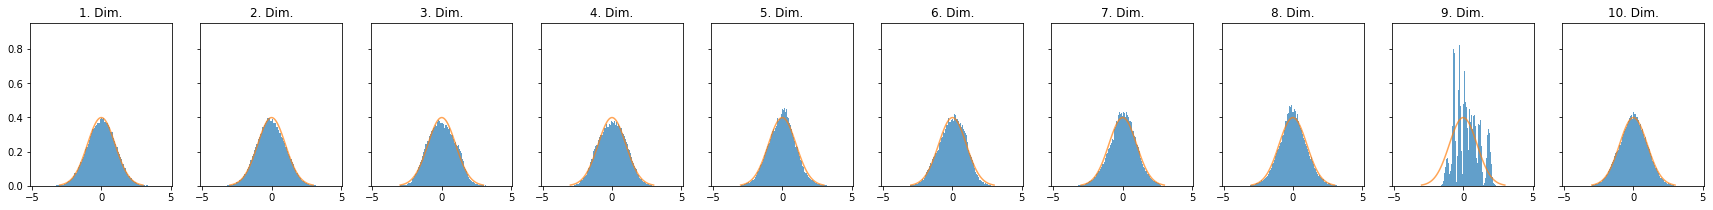
\includegraphics[width=\textwidth]{images/latent_space_entanglement/vae_dsprites_lf_10000_dist.png}
    \caption[VAE Latent Space Distribution - dSprites]{Posterior distribution of \ac{VAE} with reconstruction term weight 10,000 on 73,728 dSprites images from the validation set in 100 bins}
    \label{fig:10000_vae_latent_space_distribution}
\end{figure}

Figure~\ref{fig:10000_vae_latent_space_distribution} shows the posterior distributions of dSprites validation images.
The ninth dimension is far less Gaussian than the other nine dimensions.
As \say{object shape} is the only categorical factor of variation, one could assume that the ninth dimension encodes \say{object shape}.
However, the graph shows seven peaks in the ninth dimension, while there are only three distinct shapes in the dataset.

\begin{figure}
    \centering
    \begin{subfigure}{\textwidth}
        \centering
        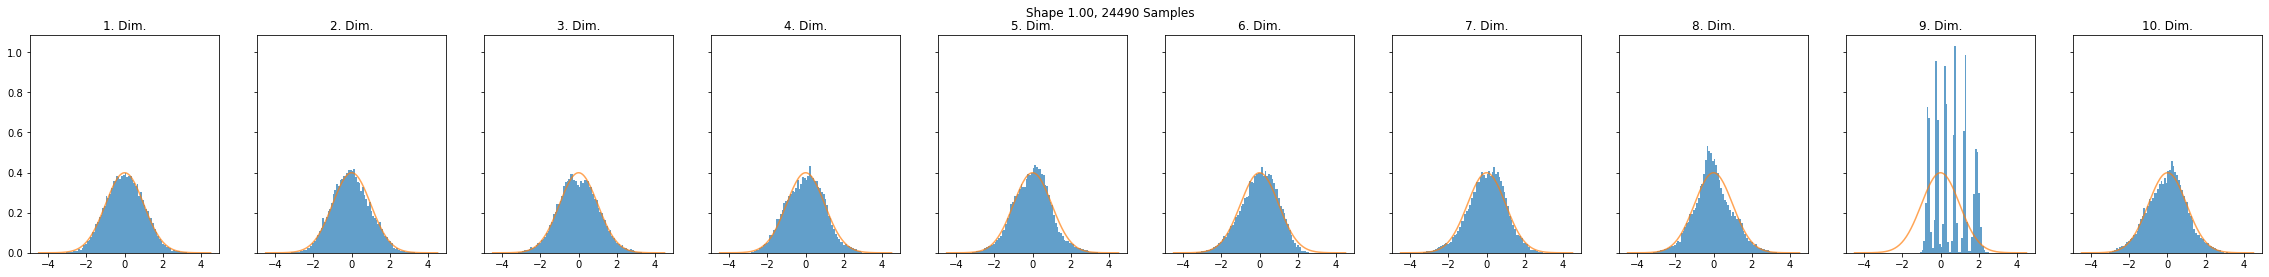
\includegraphics[width=\textwidth]{images/latent_space_entanglement/vae_dsprites_lf_10000_dist_shape_1.png}
        \caption{Latent space distribution of images with shape \textit{Square}}
    \end{subfigure}
    \begin{subfigure}{\textwidth}
        \centering
        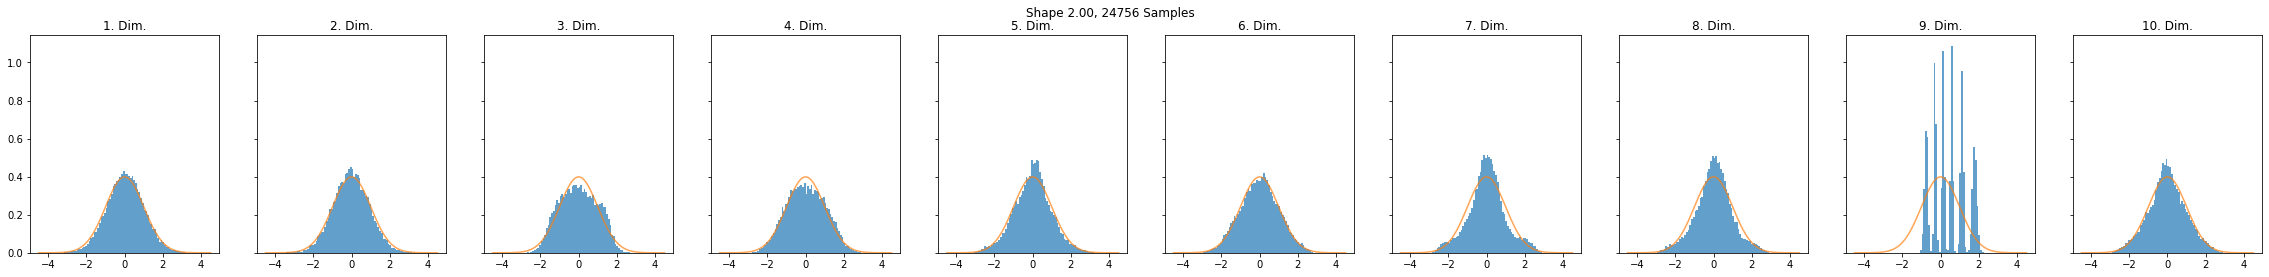
\includegraphics[width=\textwidth]{images/latent_space_entanglement/vae_dsprites_lf_10000_dist_shape_2.png}
        \caption{Latent space distribution of images with shape \textit{Ellipse}}
    \end{subfigure}
    \begin{subfigure}{\textwidth}
        \centering
        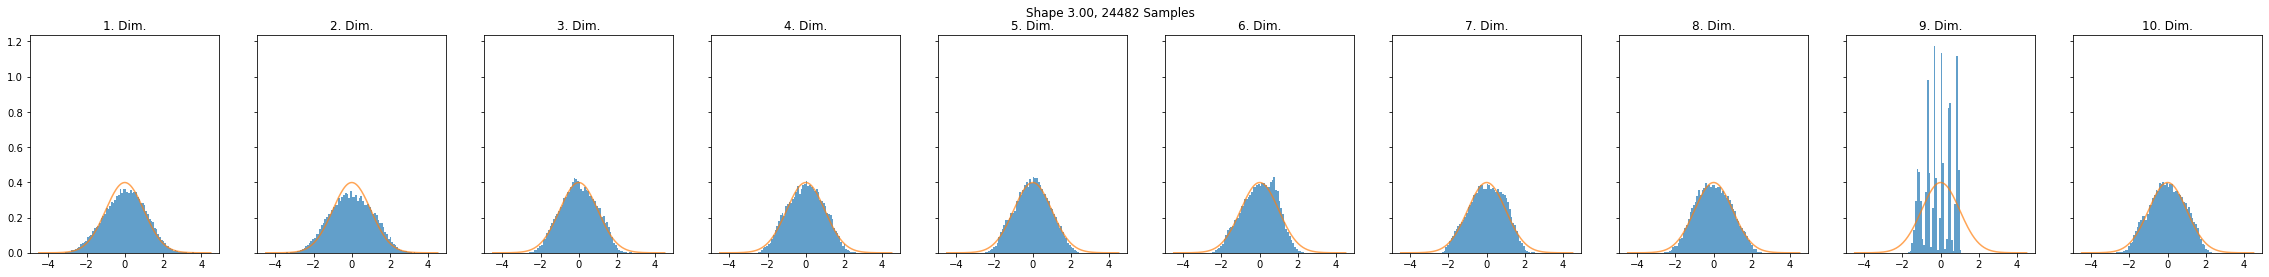
\includegraphics[width=\textwidth]{images/latent_space_entanglement/vae_dsprites_lf_10000_dist_shape_3.png}
        \caption{Latent space distribution of images with shape \textit{Heart}}
    \end{subfigure}
    \caption[VAE Latent Space Distribution - dSprites Shapes]{Histogram of dSprites images with a certain shape from the validation set in 100 bins}
    \label{fig:10000_vae_latent_space_distribution_shapes}
\end{figure}

Figure~\ref{fig:10000_vae_latent_space_distribution_shapes} shows the distribution of images with a particular shape.
Even though there is some difference between the plots, the $\mu$-values in the ninth dimension still are assigned to different and distinct areas.
The \textit{shape} alone does not explain the sharp peaks in the ninth dimension.

\begin{figure}
    \centering
    \begin{subfigure}{\textwidth}
        \centering
        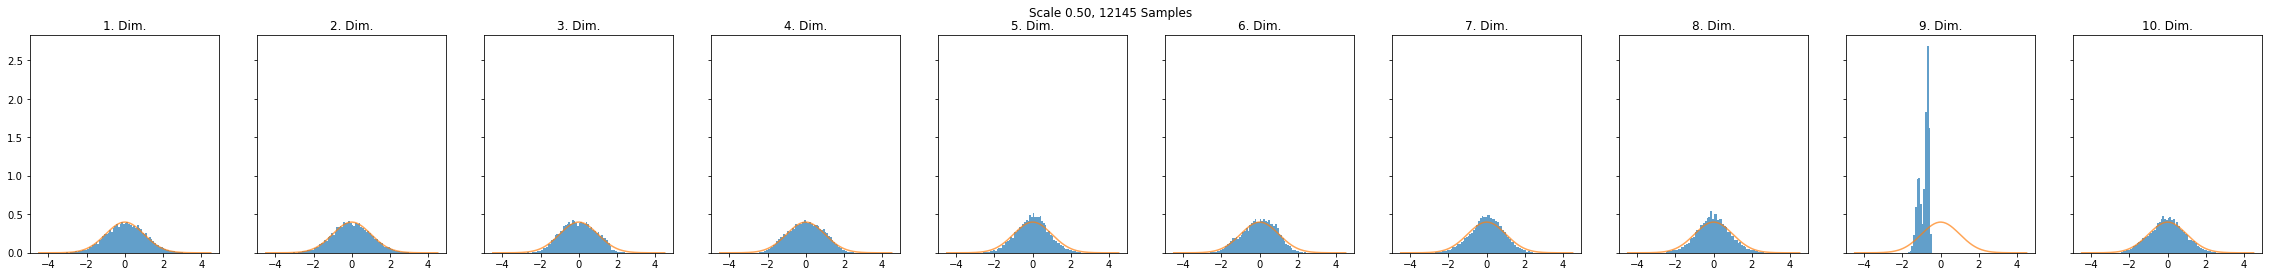
\includegraphics[width=\textwidth]{images/latent_space_entanglement/vae_dsprites_lf_10000_dist_scale_0_5.png}
        \caption{Latent space distribution of images with scale = 0.5}
    \end{subfigure}
    \begin{subfigure}{\textwidth}
        \centering
        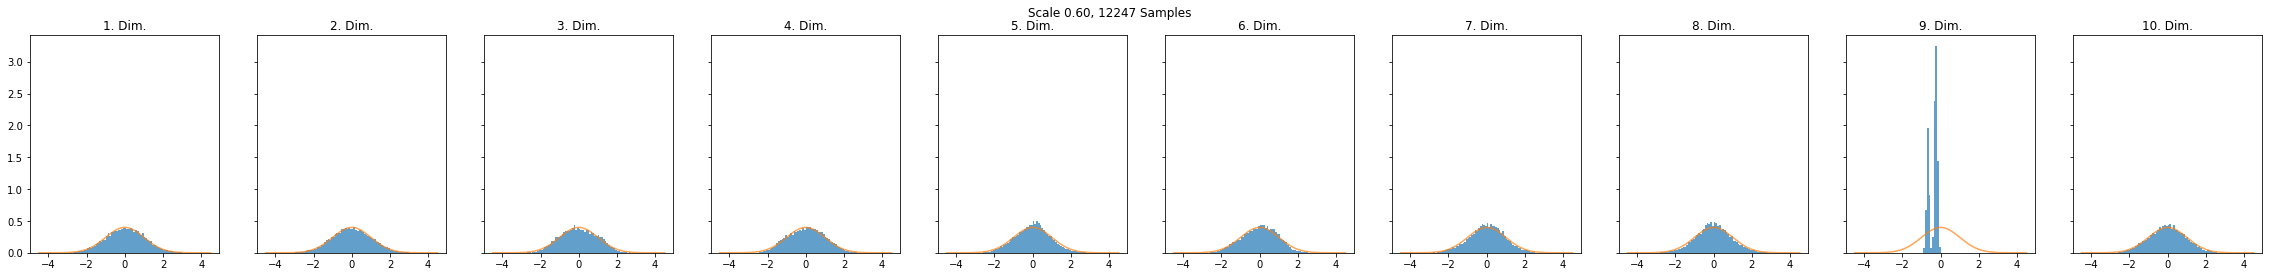
\includegraphics[width=\textwidth]{images/latent_space_entanglement/vae_dsprites_lf_10000_dist_scale_0_6.png}
        \caption{Latent space distribution of images with scale = 0.6}
    \end{subfigure}
    \begin{subfigure}{\textwidth}
        \centering
        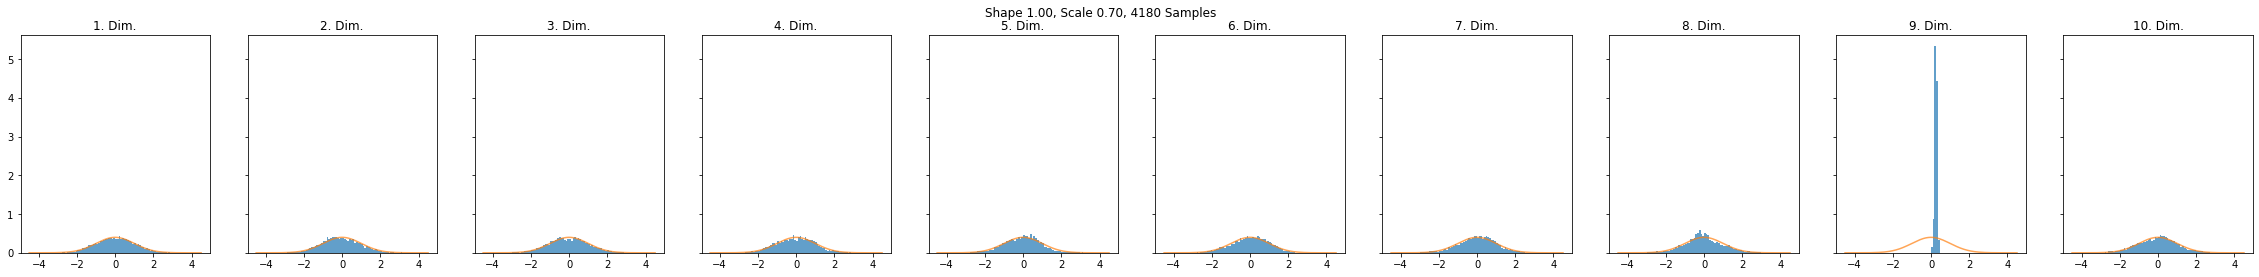
\includegraphics[width=\textwidth]{images/latent_space_entanglement/vae_dsprites_lf_10000_dist_scale_0_7.png}
        \caption{Latent space distribution of images with scale = 0.7}
    \end{subfigure}
    \begin{subfigure}{\textwidth}
        \centering
        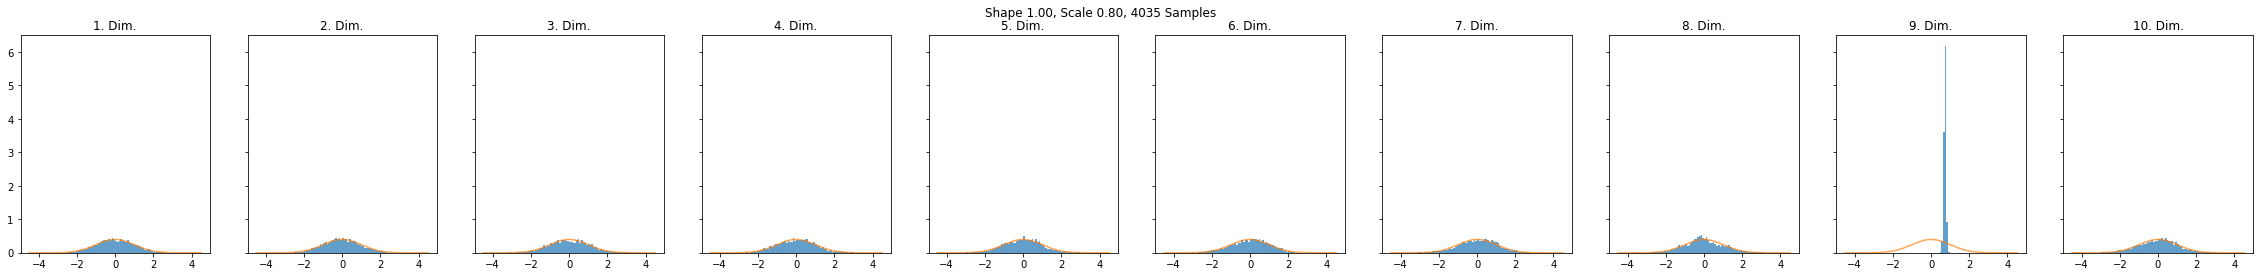
\includegraphics[width=\textwidth]{images/latent_space_entanglement/vae_dsprites_lf_10000_dist_scale_0_8.png}
        \caption{Latent space distribution of images with scale = 0.8}
    \end{subfigure}
    \begin{subfigure}{\textwidth}
        \centering
        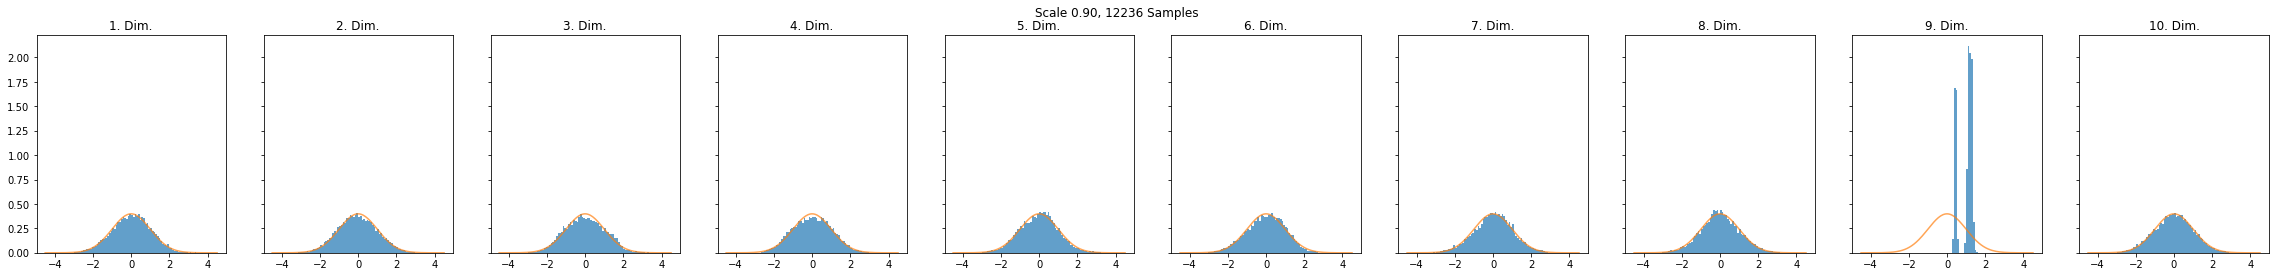
\includegraphics[width=\textwidth]{images/latent_space_entanglement/vae_dsprites_lf_10000_dist_scale_0_9.png}
        \caption{Latent space distribution of images with shape scale = 0.9}
    \end{subfigure}
    \begin{subfigure}{\textwidth}
        \centering
        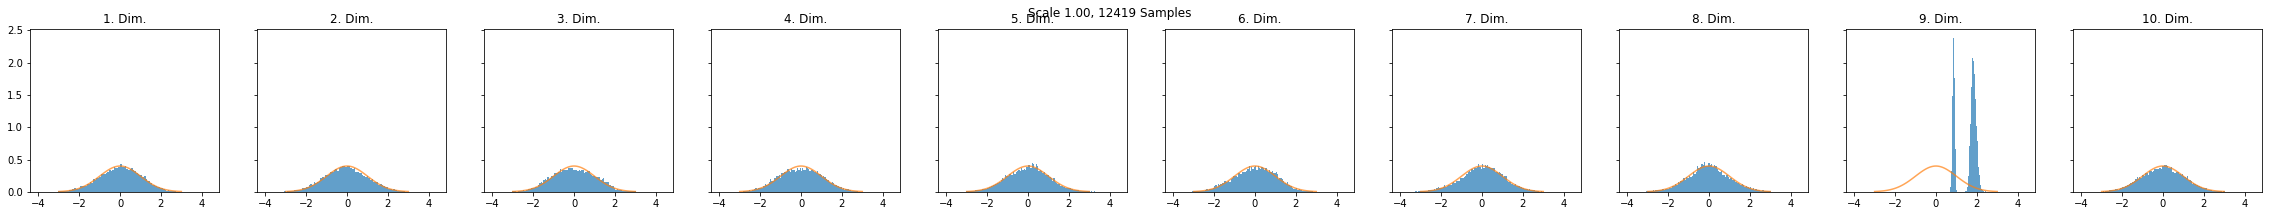
\includegraphics[width=\textwidth]{images/latent_space_entanglement/vae_dsprites_lf_10000_dist_scale_1_0.png}
        \caption{Latent space distribution of images with shape scale = 1.0}
    \end{subfigure}
    \caption[VAE Latent Space Distribution - dSprites Scales]{Posterior distribution for dSprites images with a certain scale from the validation set in 100 bins}
    \label{fig:10000_vae_latent_space_distribution_scales}
\end{figure}

Consider Figure~\ref{fig:10000_vae_latent_space_distribution_scales}.
It shows distributions of images grouped by their scale.
Images in dSprites are scaled by six distinct factors evenly chosen from $[0.5; 1.0]$.
The scale values in the dSprites dataset are six distinct values in the range from 0.5 to 1.0.
A \ac{VAE} model with a too strong reconstruction term does not learn to interpolate between these values but assigns them distinct areas in the latent space.

Grouping images by their scale \textit{and} shape explains the distinct peaks in the ninth dimension (see Figure~\ref{fig:10000_vae_latent_space_distribution_scales_and_shapes}).
Each shape has a distinct peak in the ninth dimension.
However, the peaks of shapes \textit{Ellipse} and \textit{Square} superpose.
When plotting all three shapes together, a small peak (\textit{Heart}) and a big peak (\textit{Ellipse} and \textit{Square}) can be observed.

\begin{figure}
    \centering
    \begin{subfigure}{\textwidth}
        \centering
        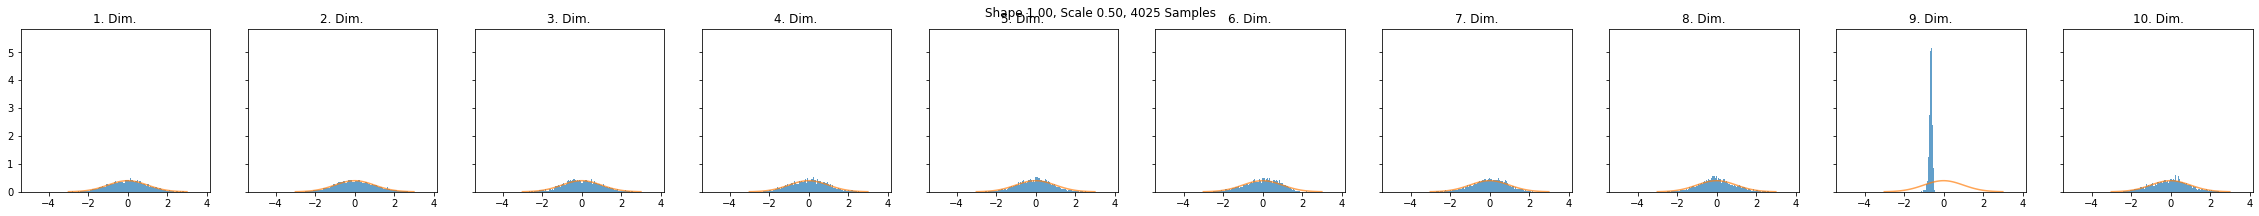
\includegraphics[width=\textwidth]{images/latent_space_entanglement/vae_dsprites_lf_10000_dist_shape_1_scale_0_5.png}
        \caption{Latent space distribution of images with scale = 0.5 and shape \textit{Square}}
    \end{subfigure}
    \begin{subfigure}{\textwidth}
        \centering
        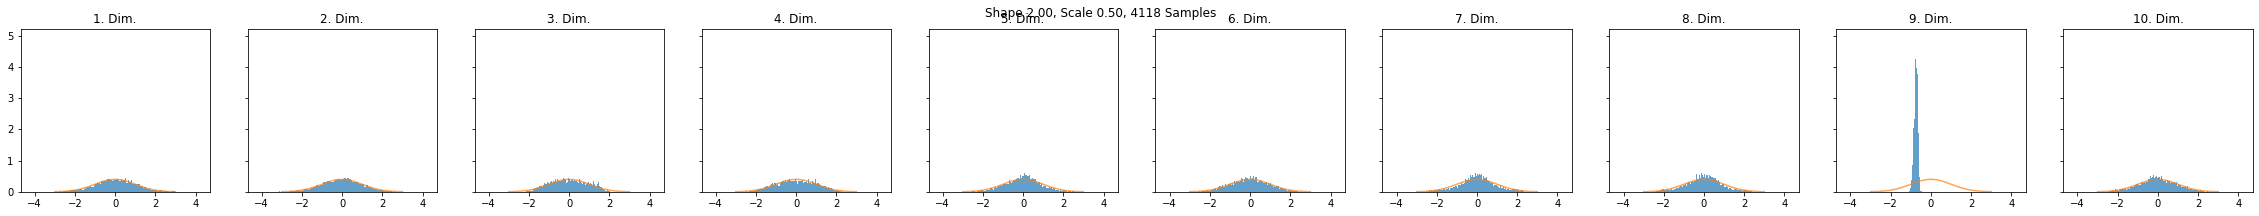
\includegraphics[width=\textwidth]{images/latent_space_entanglement/vae_dsprites_lf_10000_dist_shape_2_scale_0_5.png}
        \caption{Latent space distribution of images with scale = 0.5 and shape \textit{Ellipse}}
    \end{subfigure}
    \begin{subfigure}{\textwidth}
        \centering
        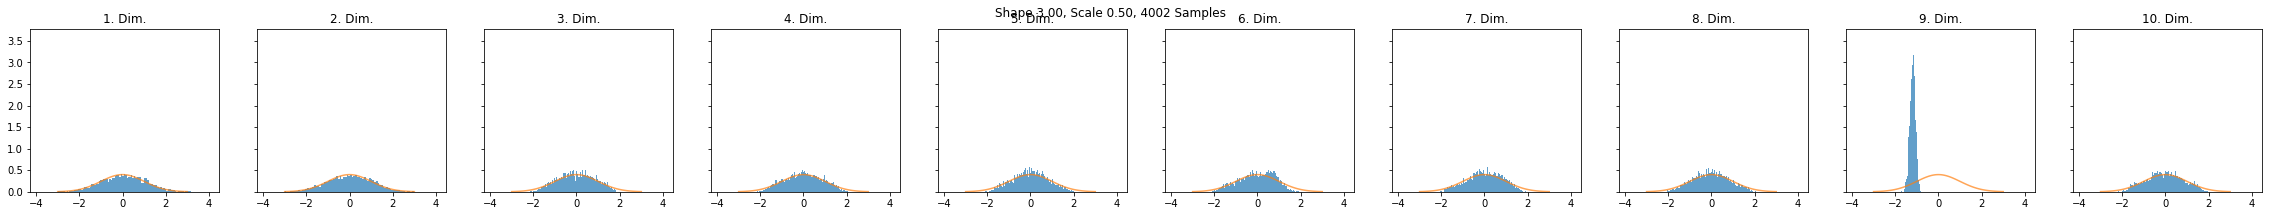
\includegraphics[width=\textwidth]{images/latent_space_entanglement/vae_dsprites_lf_10000_dist_shape_3_scale_0_5.png}
        \caption{Latent space distribution of images with scale = 0.5 and shape \textit{Heart}}
    \end{subfigure}
    \caption[VAE Latent Space Distribution - dSprites Scale and Shapes]{Posterior distribution for dSprites images with scale = 0.5 and different shapes from the validation set in 100 bins}
    \label{fig:10000_vae_latent_space_distribution_scales_and_shapes}
\end{figure}

Furthermore, the model seems to learn a hierarchical clustering in the ninth dimension.
\textit{Shape} appears to be a sub-cluster of \textit{Scale}.
This sub-clustering leads to highly entangled latent space and a highly un-Gaussian distribution.
However, it allows us to violate the \ac{KL}-term in favor of the reconstruction term in just one instead of two dimensions.

\begin{figure}
    \centering
    \begin{subfigure}{\textwidth}
        \centering
        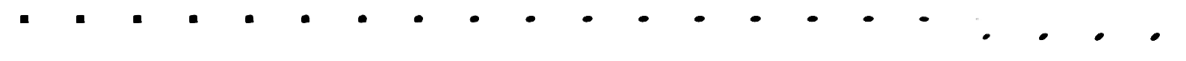
\includegraphics[width=\textwidth]{images/latent_space_entanglement/vae_10000_traverse_square_ellipse.png}
        \caption{Latent space traversal from \textit{Square} $\rightarrow$ \textit{Ellipse}}
        \label{subfig:10000_vae_latent_space_traversal_square_to_ellipse}
    \end{subfigure}
    \begin{subfigure}{\textwidth}
        \centering
        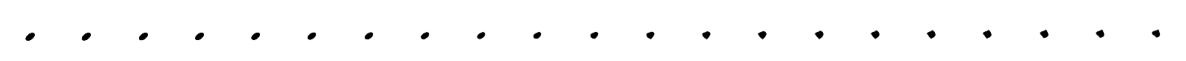
\includegraphics[width=\textwidth]{images/latent_space_entanglement/vae_10000_traverse_ellipse_heart.png}
        \caption{Latent space traversal from \textit{Ellipse} $\rightarrow$ \textit{Heart}}
    \end{subfigure}
    \begin{subfigure}{\textwidth}
        \centering
        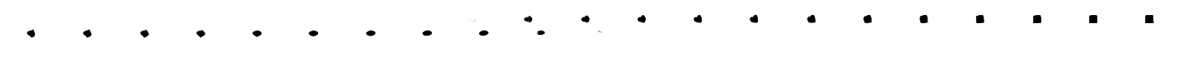
\includegraphics[width=\textwidth]{images/latent_space_entanglement/vae_10000_traverse_heart_square.png}
        \caption{Latent space traversal from \textit{Heart} $\rightarrow$ \textit{Square}}
        \label{subfig:10000_vae_latent_space_traversal_heart_to_square}
    \end{subfigure}
    \caption[VAE Latent Space Traversal - dSprites]{Latent space traversal between latent space representations of images with certain shapes for 10,000-\ac{VAE}. Color-values were inverted for this plot.}
    \label{fig:10000_vae_latent_space_traversal_shape_to_shape}
\end{figure}

Figure~\ref{fig:10000_vae_latent_space_traversal_shape_to_shape} shows generated images for a latent space traversal between different shapes\footnote{The corresponding plots for the other model can be found in Appendix~\ref{sec:additional_plots_latent_space_entanglement}.}.
For the plot, the latent representations $\bm{z}_1, \bm{z}_2$ were obtained for two $\bm{x}_i$s with identical parameters except for the shape.
Figure~\ref{fig:10000_vae_latent_space_traversal_shape_to_shape} shows the reconstructions of 21 evenly spaced points on the line segment between $\bm{z}_1$ and $\bm{z}_2$.
It shows the high degree of latent space entanglement: sudden position changes (Figure~\ref{subfig:10000_vae_latent_space_traversal_square_to_ellipse}) or the sudden emergence of new objects (Figure~\ref{subfig:10000_vae_latent_space_traversal_heart_to_square}).

Obtaining $\bm{z}$ by fixing only the shape and the scale for an $\bm{x}_i$ and averaging over all other configurations was unsuccessful.
Based on the cluster analysis, not fixing the scale would easily result in regions with low probability density.
It leads to empty images as it probably leads to $\bm{z}_i$s in regions of the latent space with low probability density.
Furthermore, for the latent space traversal shown in Figure~\ref{fig:10000_vae_latent_space_traversal_shape_to_shape}, it was possible to always find parameter combinations for which the traversal lead to empty images in the middle of the line segment.

\begin{figure}
    \centering
    \begin{subfigure}{\textwidth}
        \centering
        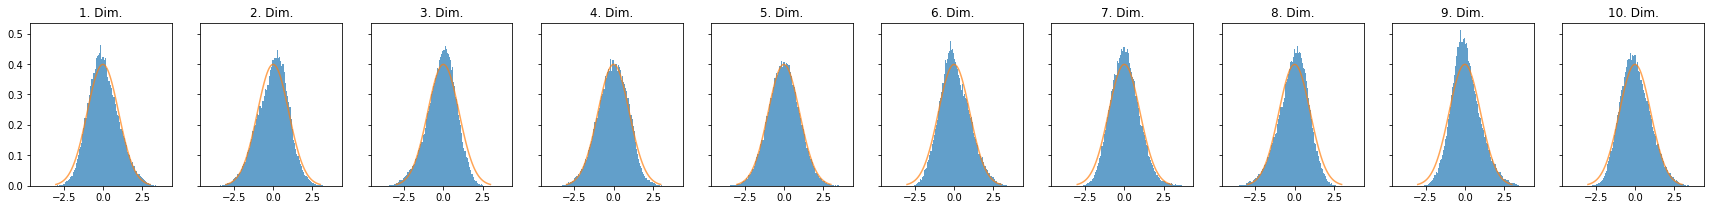
\includegraphics[width=\textwidth]{images/latent_space_entanglement/vae_dsprites_lf_7500_dist.png}
        \caption{Reconstruction term weight 7,500}
    \end{subfigure}
    \begin{subfigure}{\textwidth}
        \centering
        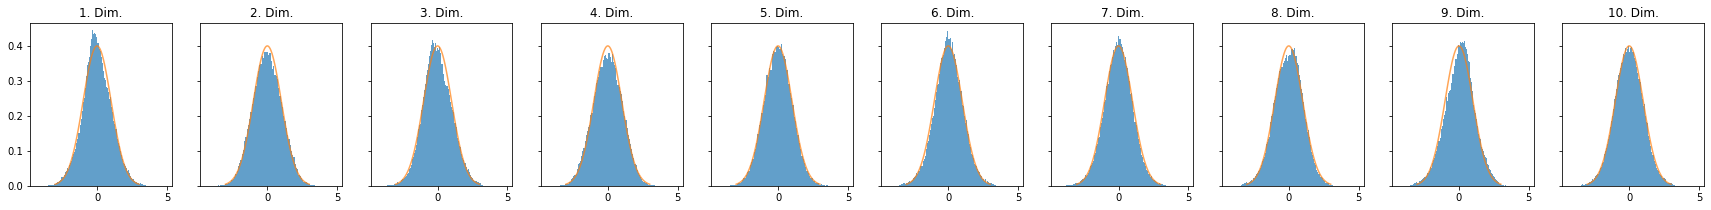
\includegraphics[width=\textwidth]{images/latent_space_entanglement/vae_dsprites_lf_6250_dist.png}
        \caption{Reconstruction term weight 6,250}
    \end{subfigure}
    \begin{subfigure}{\textwidth}
        \centering
        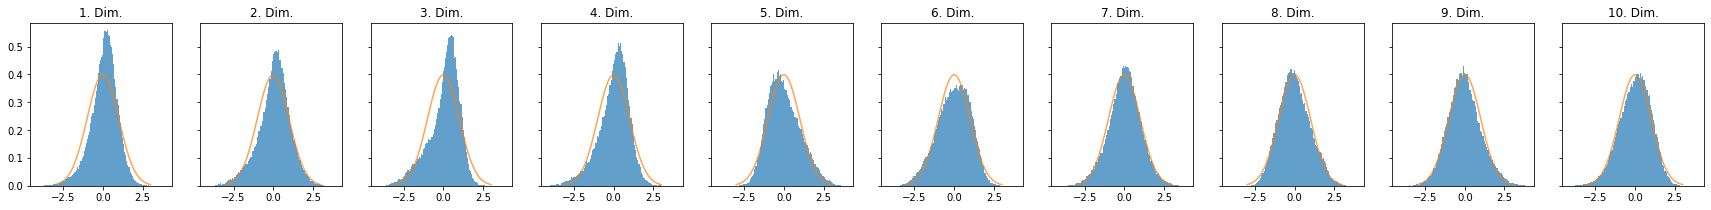
\includegraphics[width=\textwidth]{images/latent_space_entanglement/vae_dsprites_lf_5000_dist.png}
        \caption{Reconstruction term weight 5,000}
    \end{subfigure}
    \begin{subfigure}{\textwidth}
        \centering
        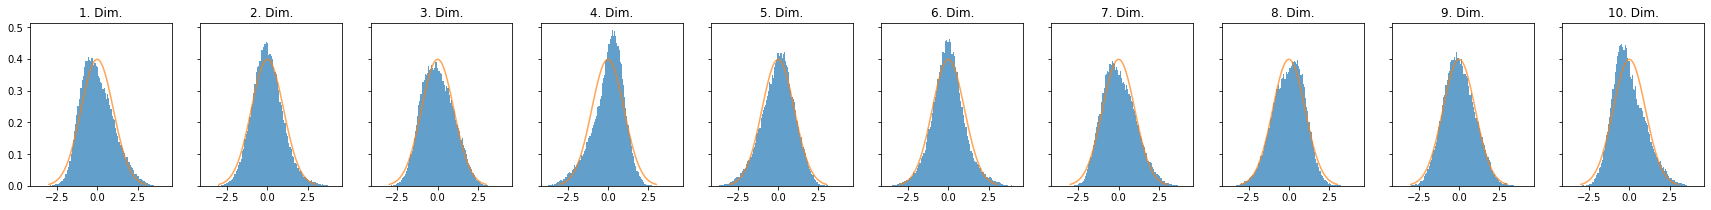
\includegraphics[width=\textwidth]{images/latent_space_entanglement/vae_dsprites_lf_3750_dist.png}
        \caption{Reconstruction term weight 3,750}
    \end{subfigure}
    \caption[VAE Latent Space Distribution - Different Reconstruction Term Weights]{Posterior distribution of VAE with different reconstruction terms weights for 73,728 dSprites images from the validation set in 100 bins}
    \label{fig:7500_5000_vae_latent_space_distribution_scales_and_shapes}
\end{figure}

Figure~\ref{fig:7500_5000_vae_latent_space_distribution_scales_and_shapes} shows the latent space distribution of \acp{VAE} with a reduced reconstruction term weight, i.e., an increase in \ac{KL-divergence} term weight.
The histograms are more Gaussian, and the \ac{KL-divergence} on the validation set decreased from 22.744 (10,000-\ac{VAE}) to 22.271 (7,500-\ac{VAE}), 19.399 (6,250-\ac{VAE}), 18.172 (5,000-\ac{VAE}), and 16.018 (3,750-\ac{VAE}).
The difference between 10,000-\ac{VAE} and 7,500-\ac{VAE} is small on the validation data, whereas the decrease in \ac{KL-divergence} is higher for 6,250-\ac{VAE}, 5,000-\ac{VAE}, and 3,750-\ac{VAE}.

To quantify the level of latent space disentanglement, the \ac{PPL}\footnote{See Section~\ref{subsec:feature-disentanglement}.} for the latent spaces of the \acp{VAE} (10,000, 7,500, 6,250, 5,000, 3,750) is computed.
The perceptual loss is obtained by a \ac{CNN}, trained to predict dSprites object categories\footnote{The model architecture can be found in Appendix~\ref{sec:appendix_feature_extraction_network_ppl_dsprites}, the features are extracted in \say{conv2d\_94}. The model was trained for one epoch using categorical crossentropy with the Adam optimizer with an initial learning rate of 0.1. The model achieved a top-1 accuracy of 0.8 on the validation set.}.
The \ac{PPL} was computed for 50 different random seeds.
Each of these \ac{PPL}-computations interpolated at 100 random steps (dependent on the random seed).

\begin{table}
    \centering
    \begin{tabular}{lrr}
        \toprule
        Model           & mean \ac{PPL} & standard deviation \\
        \midrule
        10,000-\ac{VAE} & 936.257       & 779.098            \\
        7,500-\ac{VAE}  & 2834.674      & 567.933            \\
        6,250-\ac{VAE}  & 4498.156      & 1091.255           \\
        5,000-\ac{VAE}  & 173.533       & 35.896             \\
        3,750-\ac{VAE}  & 258.326       & 49.117             \\
        \bottomrule
    \end{tabular}
    \caption[dSprites-VAEs: Perceptual Path Lengths]{Perceptual path lengths for the different models latent spaces}
    \label{tab:ppl-dsprites}
\end{table}

Table~\ref{tab:ppl-dsprites} shows the mean \ac{PPL} values and their standard deviations.
A two-sided Wilcoxon rank-sum test for the differences in the model's \acp{PPL} yielded $p$-values $< 10^{-29}$ in all cases.
The 10,000-\ac{VAE}'s \ac{PPL} is lower than for 7,500-\ac{VAE} or 6,250-\ac{VAE}.

This can be explained by the vast regions of low probability density in the posterior distribution.
For 10,000-\ac{VAE}, it is likely to produce images that are almost entirely black for some random point in the latent space.
Only a few regions in the latent space produce reasonable images.
A neighboring point in the latent space will probably also produce a black image, leading to a low perceptual loss.
As the reconstruction term weight is lowered (7,500-\ac{VAE} and 6,250-\ac{VAE}), the probability of generating some image and, therefore, the \ac{PPL} increases.
For 5,000-\ac{VAE} and 3,750-\ac{VAE}, finally, the latent space is sufficiently disentangled.
Again, this leads to a low \ac{PPL}.

The standard deviation of the \acp{PPL} supports this argumentation.
Consider 6,250-\ac{VAE}.
Here, generating some image for a random point in the latent space is already quite likely.
Nevertheless, there are still \say{enough} regions producing black images.
For these black regions, the \ac{PPL} is low, just like for 10,000-\ac{VAE}.
For the points producing images, the \ac{PPL} is high, because the latent space still is entangled.
This causes a high standard deviation.

The previous observations have some implications for the application of the \ac{PPL}.
First, the latent space needs to be approximately Gaussian for the \ac{PPL} to produce interpretable results.
Second, if the latent space is Gaussian, the standard deviation should be observed.
A too high standard deviation is evidence that there are regions of low probability density in the latent space.
The \ac{PPL} standard deviation could be a measure of this.

\subsection{Latent Space Analysis}\label{subsec:model-generated-samples}

\acp{VAE} and \acp{VLAE} force the latent space to approximate a standard normal distribution.
However, latent space disentanglement\footnote{See Section~\ref{subsec:feature-disentanglement}.} and latent space separability\footnote{See Section~\ref{subsec:feature-separability}.} require the latent space also to learn factors of variation in different (linear) sub-spaces.
The following sections explore feature learning in the latent space and answer by how far \acp{VAE} and \acp{VLAE} satisfy the requirements of latent space disentanglement and separability.

\subsubsection{Latent Space Embeddings}\label{subsubsec:latent_space_embeddings}

\paragraph{\textsc{Mnist}}

Figures~\ref{fig:vae_latent_space_mnist} and~\ref{fig:vlae_latent_space_mnist} show the latent spaces of \ac{VAE} and \ac{VLAE} trained on the \textsc{Mnist} dataset (\textsc{Mnist}-\ac{VAE} and \textsc{Mnist}-\ac{VLAE}, see Section~\ref{subsec:models}).
For \textsc{Mnist}-\ac{VAE}, there is only one latent space while there are three for \textsc{Mnist}-\ac{VLAE}.
The embeddings are colored by different means, employing information from Morpho-\textsc{Mnist} (see Section~\ref{subsubsec:morphomnist}) and the digit identity information provided by \textsc{Mnist} itself.

As discussed in Section~\ref{subsubsec:representation_learning}, the \ac{VLAE} aims at learning \say{hierarchical disentangled representation}~\citep{zhao2017learning}.
The lower embedding layers of such a model trained on \textsc{Mnist} (see Section~\ref{subsubsec:mnist}) encode features such as stroke width, digit width, and digit tilt, whereas the highest layer mainly learns digit identity~\citep{zhao2017learning}.

Incorporating the additional labels provided by Morpho-\textsc{Mnist} analyzing to what extent the lower layers learn which morphological features of \textsc{MNIST}.
The morphological attributes, however, are not equally distributed for all digits.
The mean stroke length and the digit width, for example, have a low mean value for the digit \say{1} (see Figure~\ref{fig:morpho_mnist_distribution}).
Therefore, it should be possible to almost uniquely identify digit \say{1} identity by just considering the stroke length or the digit width.
Other attributes, such as stroke thickness, digit slant, and digit height, are more evenly distributed (see Figure~\ref{fig:morpho_mnist_distribution}).

Consider Figure~\ref{subfig:vlae_mnist_latent_space_z_1_slant} showing the embedding layer $\bm{z}_1$ colored by digit slant.
Figure~\ref{fig:morpho_mnist_distribution} shows that the mean of the attribute \textit{slant} is quite evenly distributed.
The color gradient in Figure~\ref{subfig:vlae_mnist_latent_space_z_1_slant}, therefore, indicates that the VLAE learns the morphological attribute instead of just showing the class identity, encoded using another morphological attribute that correlates with class identity.

For Figure~\ref{subfig:vlae_mnist_latent_space_z_1_width}, the situation is different.
The noticeable dark-purple cluster in the top left correlates with dark-purple points in Figure~\ref{subfig:vlae_mnist_latent_space_z_1_identity} that encode images with label \say{1}.
For digit width, however, \say{1} is an outlier (see Figure~\ref{fig:morpho_mnist_distribution}), and a small digit width, therefore, is a reliable indicator for a digit identity of \say{1}.
Nonetheless, overall digit identity does not seem to be encoded strongly by $\bm{z}_1$ (see Figure~\ref{subfig:vlae_mnist_latent_space_z_1_identity}).

\begin{figure}
    \centering
    \begin{subfigure}{.32\textwidth}
        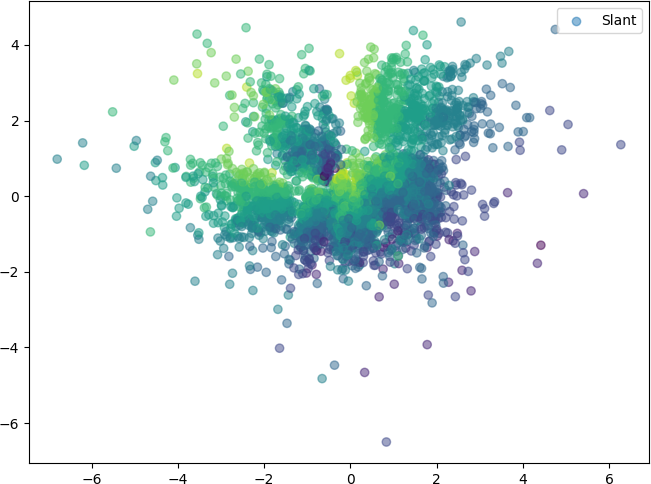
\includegraphics[width=\textwidth]{images/latent_spaces/mnist/vae/embeddings_mu_0.png}
        \caption{Latent space colored by digit slant}
        \label{subfig:vae_mnist_latent_space_slant}
    \end{subfigure}
    \hfill
    \begin{subfigure}{.32\textwidth}
        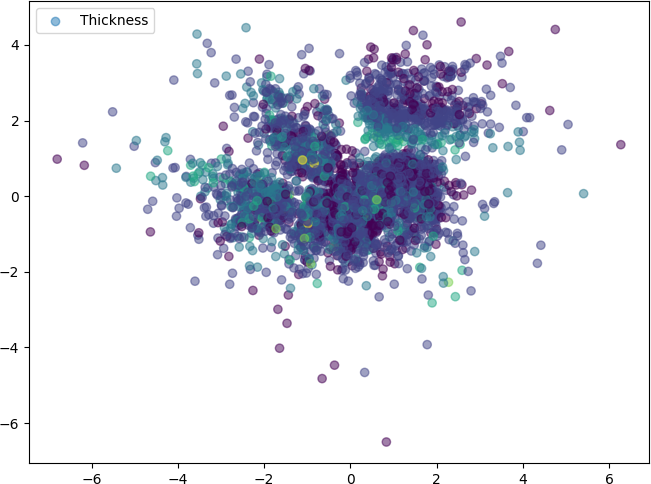
\includegraphics[width=\textwidth]{images/latent_spaces/mnist/vae/embeddings_mu_1.png}
        \caption{Latent space colored by digit thickness}
        \label{subfig:vae_mnist_latent_space_thickness}
    \end{subfigure}
    \hfill
    \begin{subfigure}{.32\textwidth}
        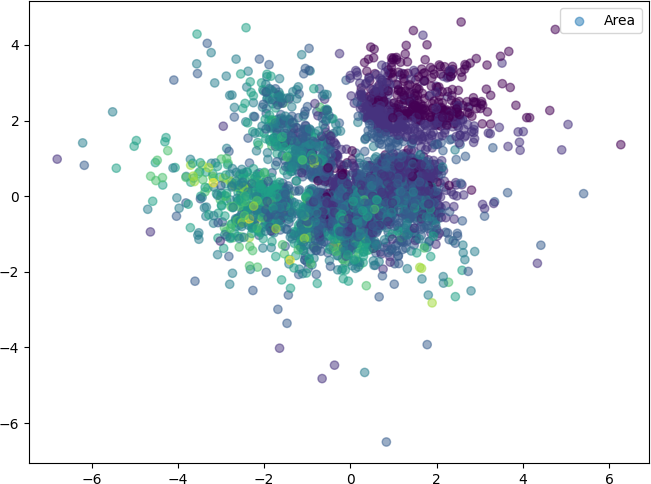
\includegraphics[width=\textwidth]{images/latent_spaces/mnist/vae/embeddings_mu_2.png}
        \caption{Latent space colored by digit area}
        \label{subfig:vae_mnist_latent_space_area}
    \end{subfigure}
    \hfill
    \begin{subfigure}{.24\textwidth}
        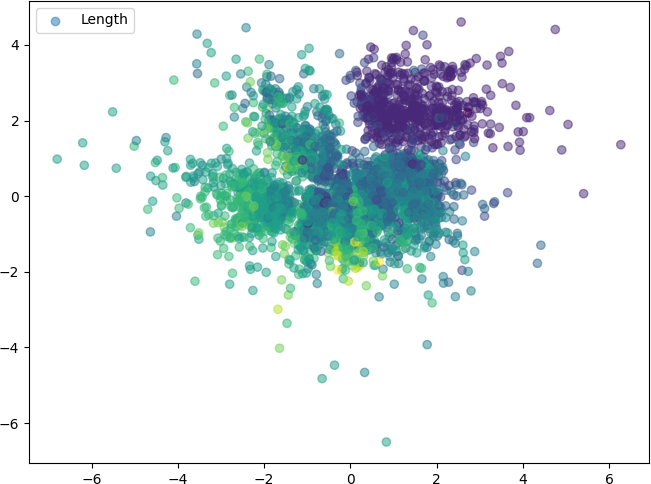
\includegraphics[width=\textwidth]{images/latent_spaces/mnist/vae/embeddings_mu_3.png}
        \caption{Latent space colored by digit length}
        \label{subfig:vae_mnist_latent_space_length}
    \end{subfigure}
    \hfill
    \begin{subfigure}{.24\textwidth}
        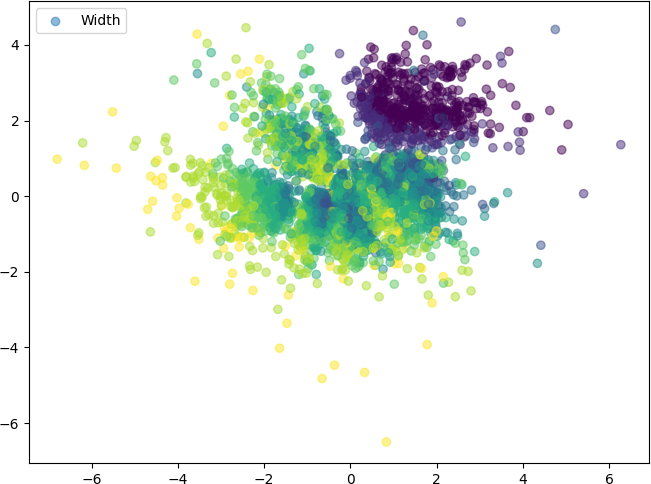
\includegraphics[width=\textwidth]{images/latent_spaces/mnist/vae/embeddings_mu_4.png}
        \caption{Latent space colored by digit width}
        \label{subfig:vae_mnist_latent_space_width}
    \end{subfigure}
    \hfill
    \begin{subfigure}{.24\textwidth}
        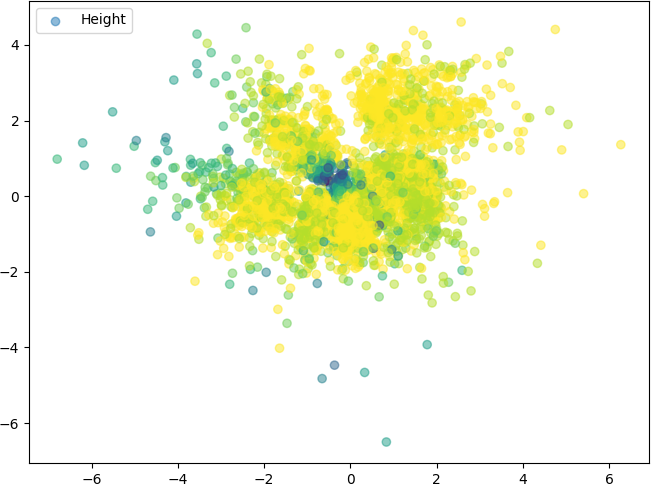
\includegraphics[width=\textwidth]{images/latent_spaces/mnist/vae/embeddings_mu_5.png}
        \caption{Latent space colored by digit height}
        \label{subfig:vae_mnist_latent_space_height}
    \end{subfigure}
    \hfill
    \begin{subfigure}{.24\textwidth}
        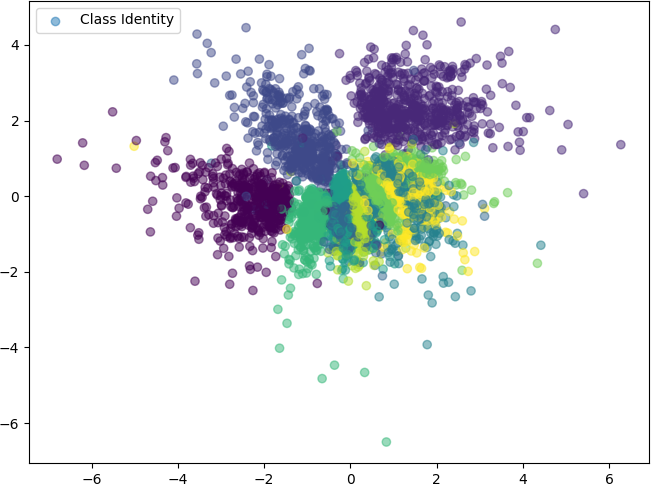
\includegraphics[width=\textwidth]{images/latent_spaces/mnist/vae/embeddings_mu_6.png}
        \caption{Latent space colored by digit identity}
        \label{subfig:vae_mnist_latent_space_identity}
    \end{subfigure}
    \caption[\textsc{Mnist}-VAE - Latent Space]{Latent space colored by different means of \textsc{Mnist}-\ac{VAE}}
    \label{fig:vae_latent_space_mnist}
\end{figure}

\begin{landscape}
    \begin{figure}
        \centering
        \foreach \i in {1,2,3}{
        \begin{adjustbox}{valign=T}
            \begin{subfigure}{.19\textwidth}
                \includegraphics[width=\textwidth]{images/latent_spaces/mnist/vlae/embeddings_mu_\i_0.png}
                \caption{$z_{\i}$: digit slant}
                \label{subfig:vlae_mnist_latent_space_z_\i_slant}
            \end{subfigure}
        \end{adjustbox}
        \hfill
        \begin{adjustbox}{valign=T}
            \begin{subfigure}{.19\textwidth}
                \includegraphics[width=\textwidth]{images/latent_spaces/mnist/vlae/embeddings_mu_\i_1.png}
                \caption{$z_{\i}$: digit thickness}
                \label{subfig:vlae_mnist_latent_space_z_\i_thickness}
            \end{subfigure}
        \end{adjustbox}
        \hfill
        \begin{adjustbox}{valign=T}
            \begin{subfigure}{.19\textwidth}
                \includegraphics[width=\textwidth]{images/latent_spaces/mnist/vlae/embeddings_mu_\i_2.png}
                \caption{$z_{\i}$: digit area}
                \label{subfig:vlae_mnist_latent_space_z_\i_area}
            \end{subfigure}
        \end{adjustbox}
        \hfill
        \begin{adjustbox}{valign=T}
            \begin{subfigure}{.19\textwidth}
                \includegraphics[width=\textwidth]{images/latent_spaces/mnist/vlae/embeddings_mu_\i_3.png}
                \caption{$z_{\i}$: digit length}
                \label{subfig:vlae_mnist_latent_space_z_\i_length}
            \end{subfigure}
        \end{adjustbox}
        \hfill
        \begin{adjustbox}{valign=T}
            \begin{subfigure}{.19\textwidth}
                \includegraphics[width=\textwidth]{images/latent_spaces/mnist/vlae/embeddings_mu_\i_4.png}
                \caption{$z_{\i}$: digit width}
                \label{subfig:vlae_mnist_latent_space_z_\i_width}
            \end{subfigure}
        \end{adjustbox}
        \hfill
        \begin{adjustbox}{valign=T}
            \begin{subfigure}{.19\textwidth}
                \includegraphics[width=\textwidth]{images/latent_spaces/mnist/vlae/embeddings_mu_\i_5.png}
                \caption{$z_{\i}$: digit height}
                \label{subfig:vlae_mnist_latent_space_z_\i_height}
            \end{subfigure}
        \end{adjustbox}
        \hfill
        \begin{adjustbox}{valign=T}
            \begin{subfigure}{.19\textwidth}
                \includegraphics[width=\textwidth]{images/latent_spaces/mnist/vlae/embeddings_mu_\i_6.png}
                \caption{$z_{\i}$: digit identity}
                \label{subfig:vlae_mnist_latent_space_z_\i_identity}
            \end{subfigure}
        \end{adjustbox}}
        \caption[\textsc{Mnist}-VLAE Latent Space]{Latent space colored by different means of \textsc{Mnist}-\ac{VLAE}}
        \label{fig:vlae_latent_space_mnist}
    \end{figure}
\end{landscape}

Noticeable, digit identity seems to be learned in $\bm{z}_2$ and $\bm{z}_3$ (see Figures~\ref{subfig:vlae_mnist_latent_space_z_2_identity} and \ref{subfig:vlae_mnist_latent_space_z_3_identity}).
However, learning one factor of variation on two layers would be a contradiction to Figure~\ref{subfig:vlae_mnist_latent_space_traversal} and even more Figure~\ref{subfig:vlae_gan_mnist_latent_space_traversal}, showing that digit identity mainly is learned in the last embedding layer.
Albeit $\bm{z}_2$ has some influence on digit identity, this effect is not nearly as prominent as for $\bm{z}_3$ even though the clustering in Figure~\ref{subfig:vlae_mnist_latent_space_z_2_identity} seems to be almost as good as in Figure~\ref{subfig:vlae_mnist_latent_space_z_3_identity}.
It seems that the digit identity learned in $\bm{z}_2$ only supports the model generation but has a far less strong influence than $\bm{z}_3$.

All in all, \ac{VLAE} does not seem to learn entirely separable representations.
However, the less powerful network below $\bm{z}_1$ indeed seems to learn lower-level representations that also are employed when generating new images (see Figures~\ref{subfig:vlae_mnist_latent_space_traversal} and \ref{subfig:vlae_gan_mnist_latent_space_traversal}).

For \ac{VAE}, digit identity defines the shape of the latent space (Figure~\ref{subfig:vae_mnist_latent_space_identity}), leading to more prominent \say{main clusters.}
As \ac{VAE} only has one latent space, it employs subspaces to learn the lower-level factors of variation, such as slant within the main clusters (Figure~\ref{subfig:vae_mnist_latent_space_slant}).

The \ac{VAE} seems to learn an efficient encoding of most of the factors of variation as revealed by this kind of visualization even though it has a narrower information bottleneck with a two-dimensional latent space compared to the three two-dimensional latent spaces of \ac{VLAE}.

\paragraph{CelebA}

\begin{wrapfigure}[26]{R}{0.4\textwidth}
    \centering
    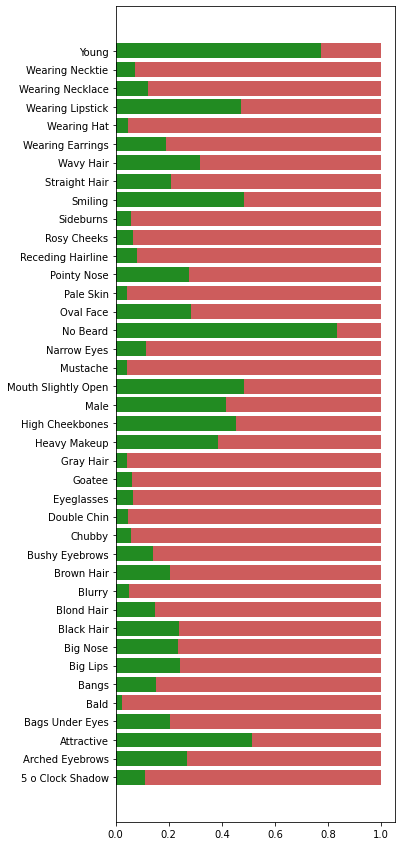
\includegraphics[height=.39\textheight]{images/latent_spaces/celeba/attribute_distribution.png}
    \caption[CelebA: Feature Distribution]{Distribution of the Binary Factors of Variation in the CelebA dataset. The green bar shows the fraction of the images where the attribute is present, the red bar where it is not present.}
    \label{fig:celeba_features_distribution}
\end{wrapfigure}

\begin{figure}
    \centering
    \begin{subfigure}{.49\textwidth}
        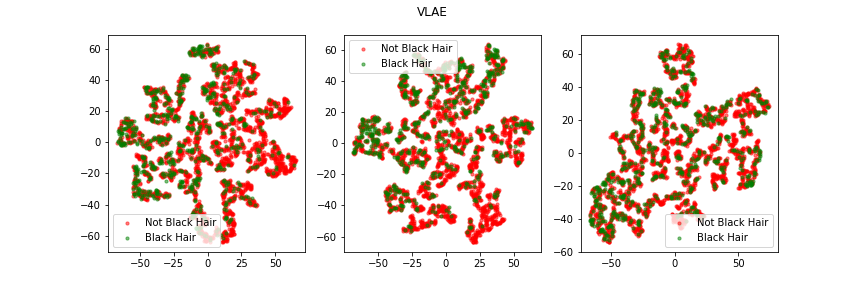
\includegraphics[width=\textwidth]{images/latent_spaces/celeba/vlae/vlae_celeba_Black_Hair.png}
        \caption{Black hair present (green) or not (red)}
        \label{subfig:latent_space_celeba_vale_colored_black_hair}
    \end{subfigure}
    \hfill
    \begin{subfigure}{.49\textwidth}
        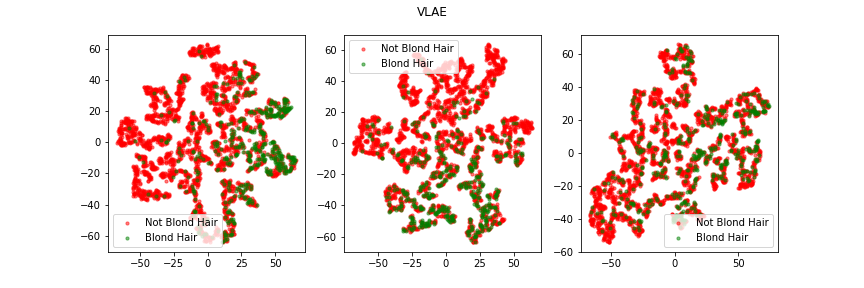
\includegraphics[width=\textwidth]{images/latent_spaces/celeba/vlae/vlae_celeba_Blond_Hair.png}
        \caption{Blond hair present (green) or not (red)}
        \label{subfig:latent_space_celeba_vale_colored_blond_hair}
    \end{subfigure}
    \begin{subfigure}{.49\textwidth}
        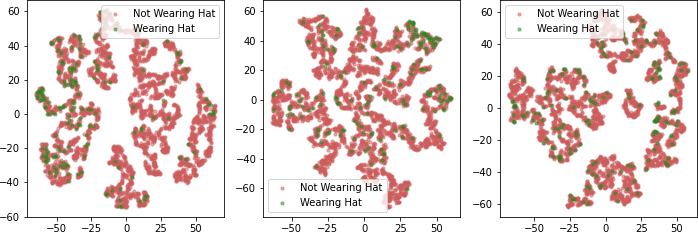
\includegraphics[width=\textwidth]{images/latent_spaces/celeba/vlae/vlae_celeba_Wearing_Hat.png}
        \caption{Wearing a hat (green) or not (red)}
        \label{subfig:latent_space_celeba_vale_colored_waring_hat}
    \end{subfigure}
    \hfill
    \begin{subfigure}{.49\textwidth}
        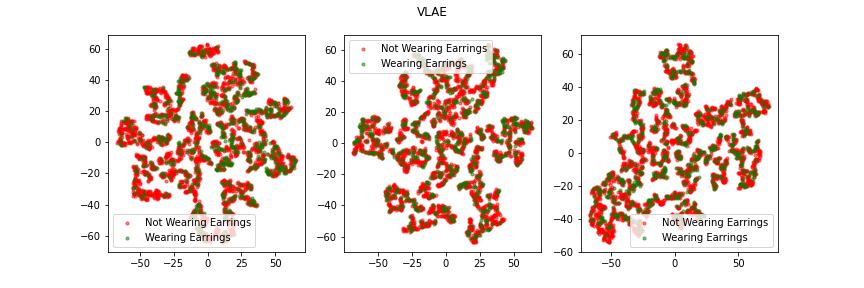
\includegraphics[width=\textwidth]{images/latent_spaces/celeba/vlae/vlae_celeba_Wearing_Earrings.png}
        \caption{Wearing earrings (green) or not (red)}
        \label{subfig:latent_space_celeba_vale_colored_wearing_earrings}
    \end{subfigure}
    \caption[VLAE Latent Space for CelebA, Curated Features]{\ac{t-SNE}-reduced Latent Space of a \ac{VLAE} trained on CelebA, colored by curated Factors of Variation (present or not present)}
    \label{fig:latent_space_celeba_vale_colored}
\end{figure}

The CelebA dataset provides binary labels for factors of variation.
Figure~\ref{fig:celeba_features_distribution} shows the distribution of the different features in the dataset.
Figure~\ref{fig:latent_space_celeba_vale_colored} shows the \ac{t-SNE}-reduced latent space of a CelebA-\ac{VLAE} (see Section~\ref{subsubsec:vlae_models}).
A green dot in the latent space indicates that the feature is present for the data point, a red point indicates that it is not present\footnote{The plots for all models and all factors of variation can be found in Appendix~\ref{subsection:appendix_celeba_latent_space}.}.

The latent space plots allow to analyze which features are learned in which layers.
For example, hair color is mainly learned in the first and second layers (see Figures~\ref{subfig:latent_space_celeba_vale_colored_black_hair} and \ref{subfig:latent_space_celeba_vale_colored_blond_hair}) because green and red dots build clusters within these layers.
Other features do not seem to be learned at all (see Figure~\ref{subfig:latent_space_celeba_vale_colored_wearing_earrings}).

CelebA provides only binary attributes, the latent space analysis is less insightful than for dSprites and Morpho-\textsc{Mnist}.
Furthermore, the models learn factors of variation that are not present in the labels (see Section~\ref{subsubsec:latent_space_traversals}).

\paragraph{dSprites}

The latent space embeddings for the dSprites dataset allow a more profound comparison of \ac{VAE} and \ac{VLAE}.
Here, the dSprites-\ac{VAE}-dim6 model (see Section~\ref{subsubsec:vae_models}) was given a six-dimensional embedding space, whereas the dSprites-\ac{VLAE}-dim2 (see Section~\ref{subsubsec:vlae_models}) model has three two-dimensional embedding spaces.
The \ac{VAE} and \ac{VLAE} approximately have the same model capacity under the assumption that \ac{VLAE} uses lower embedding layers to learn lower-level features and higher embedding layers to only learn higher-level features and that the dataset can be split in this way.
The \ac{VLAE} latent spaces were chosen two-dimensional to allow for a direct visualization of the latent space without dimensionality reduction.
As the \ac{VAE} model employs a higher-dimensional latent space, the embeddings are visualized using \ac{t-SNE} embeddings (see Figure~\ref{fig:vae_latent_space_dsprites}).

One advantage of dSprites over \textsc{Mnist} is that all factors of variation by design are independent and represented equally often, allowing a more straightforward analysis.

\begin{figure}
    \centering
    \begin{adjustbox}{valign=T}
        \begin{subfigure}{.19\textwidth}
            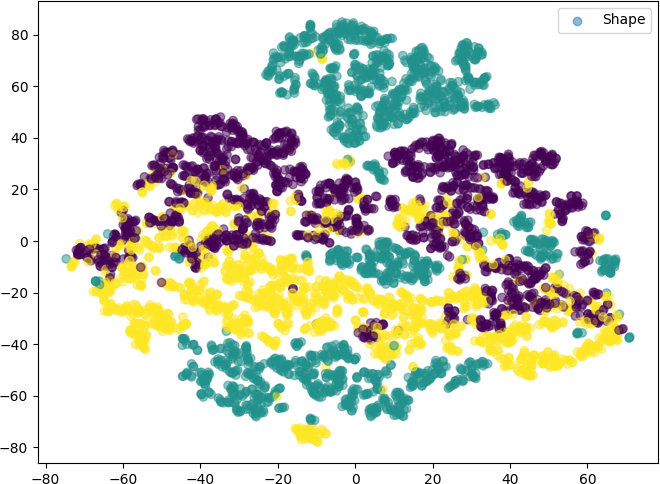
\includegraphics[width=\textwidth]{images/latent_spaces/dsprites/vae/embeddings_mu_0.png}
            \caption{Latent space colored by object shape}
        \end{subfigure}
    \end{adjustbox}
    \hfill
    \begin{adjustbox}{valign=T}
        \begin{subfigure}{.19\textwidth}
            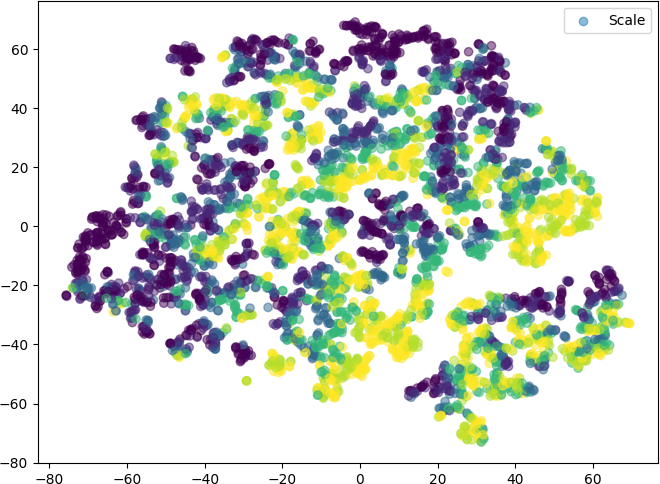
\includegraphics[width=\textwidth]{images/latent_spaces/dsprites/vae/embeddings_mu_1.png}
            \caption{Latent space colored by object scale}
            \label{subfig:vae_embedding_dsprites_scale}
        \end{subfigure}
    \end{adjustbox}
    \hfill
    \begin{adjustbox}{valign=T}
        \begin{subfigure}{.19\textwidth}
            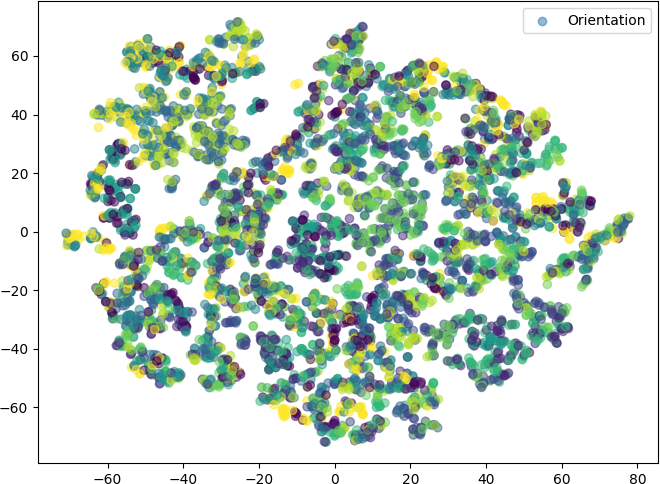
\includegraphics[width=\textwidth]{images/latent_spaces/dsprites/vae/embeddings_mu_2.png}
            \caption{Latent space colored by object orientation}
            \label{subfig:vae_embedding_dsprites_orientation}
        \end{subfigure}
    \end{adjustbox}
    \hfill
    \begin{adjustbox}{valign=T}
        \begin{subfigure}{.19\textwidth}
            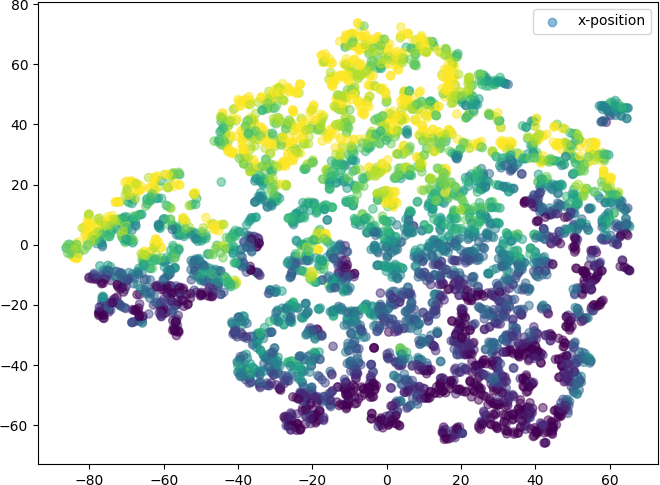
\includegraphics[width=\textwidth]{images/latent_spaces/dsprites/vae/embeddings_mu_3.png}
            \caption{Latent space colored by object $x$-position}
        \end{subfigure}
    \end{adjustbox}
    \hfill
    \begin{adjustbox}{valign=T}
        \begin{subfigure}{.19\textwidth}
            \includegraphics[width=\textwidth]{images/latent_spaces/dsprites/vae/embeddings_mu_4.png}
            \caption{Latent space colored by object $y$-position}
        \end{subfigure}
    \end{adjustbox}
    \caption[dsprites-VAE-dim6 - Latent Space]{\ac{t-SNE}-reduced latent space embeddings colored by different means of dSprites-\ac{VAE}-dim6}
    \label{fig:vae_latent_space_dsprites}
\end{figure}

\begin{figure}
    \centering
    \foreach \i in {1,2,3}{
    \begin{subfigure}{.19\textwidth}
        \includegraphics[width=\textwidth]{images/latent_spaces/dsprites/vlae/embeddings_mu_\i_0.png}
        \caption{Latent space $\bm{z}_{\i}$ colored by object shape}
        \label{subfig:vlae_embedding_z\i_dsprites_shape}
    \end{subfigure}
    \hfill
    \begin{subfigure}{.19\textwidth}
        \includegraphics[width=\textwidth]{images/latent_spaces/dsprites/vlae/embeddings_mu_\i_1.png}
        \caption{Latent space $\bm{z}_{\i}$ colored by object scale}
        \label{subfig:vlae_embedding_z\i_dsprites_scale}
    \end{subfigure}
    \hfill
    \begin{subfigure}{.19\textwidth}
        \includegraphics[width=\textwidth]{images/latent_spaces/dsprites/vlae/embeddings_mu_\i_2.png}
        \caption{Latent space $\bm{z}_{\i}$ colored by object orientation}
        \label{subfig:vlae_embedding_z\i_dsprites_orientation}
    \end{subfigure}
    \hfill
    \begin{subfigure}{.19\textwidth}
        \includegraphics[width=\textwidth]{images/latent_spaces/dsprites/vlae/embeddings_mu_\i_3.png}
        \caption{Latent space $\bm{z}_{\i}$ colored by object $x$-position}
        \label{subfig:vlae_embedding_z\i_dsprites_x_pos}
    \end{subfigure}
    \hfill
    \begin{subfigure}{.19\textwidth}
        \includegraphics[width=\textwidth]{images/latent_spaces/dsprites/vlae/embeddings_mu_\i_4.png}
        \caption{Latent space $\bm{z}_{\i}$ colored by object $y$-position}
        \label{subfig:vlae_embedding_z\i_dsprites_y_pos}
    \end{subfigure}
    }
    \caption[dsprites-VLAE-dim2 - Latent Space]{Latent space colored by different means of dSprites-\ac{VLAE}-dim2}
    \label{fig:vlae_latent_space_dsprites}
\end{figure}

Again, the \ac{VAE} builds main clusters and seems to embed the lower-level features into main clusters.
Especially the object scale seems to be a lower-level feature (see Figure~\ref{subfig:vae_embedding_dsprites_scale}).
Only object-orientation does not seem to be learned at all (see Figure~\ref{subfig:vae_embedding_dsprites_orientation}).

dsprites-\ac{VLAE}-dim2 (see Figure~\ref{fig:vlae_latent_space_dsprites}) is worse compared to dSprites-\ac{VAE}-dim6.
Again, the model learns main clusters, especially for object position (see Figures~\ref{subfig:vlae_embedding_z3_dsprites_x_pos} and~\ref{subfig:vlae_embedding_z3_dsprites_y_pos}).
Furthermore, the model learns the object scale (see Figure~\ref{subfig:vlae_embedding_z3_dsprites_scale} and \ref{subfig:vlae_embedding_z2_dsprites_scale}).
Apart from that, the model does not seem to learn other factors of variation.
The representations are not particularly disentangled.
Object position and scale are learned in all layers, but best in $z_3$.

After training 200 epochs, dSprites-\ac{VAE}-dim6 achieved a loss of 21.638 (reconstruction loss: 6.375, \ac{KL}-loss: 15.264).
In contrast, dSprites-\ac{VLAE}-dim2 achieved a loss of 47.860 (reconstruction loss: 32.813, \ac{KL}-loss: 15.047).

All in all, using a \ac{VAE} with a higher-dimensional space seems superior to the \ac{VLAE} in terms of encoding efficiency.

\subsubsection{Latent Space Explorations}\label{subsubsec:latent_space_traversals}

\subparagraph{\textsc{Mnist}}

A latent space exploration is one way to see if and how a model learns a general representation of the dataset.
Figures~\ref{fig:mnist_latent_space_traversal_vae} and \ref{fig:mnist_latent_space_traversal_vlae} show the latent space traversal of \textsc{Mnist}-\ac{VAE}\footnote{See Section~\ref{subsubsec:vae_models}.}, \textsc{Mnist}-\ac{VAE}-\ac{GAN}\footnote{See Section~\ref{subsubsec:vae_gan_models}.}, \textsc{Mnist}-\ac{VLAE}\footnote{See Section~\ref{subsubsec:vlae_models}.}, and \textsc{Mnist}-\ac{VLAE}-\ac{GAN}\footnote{See Section~\ref{subsubsec:vlae_gan_models}.}.
For the models with only one latent layer (\textsc{Mnist}-\ac{VAE} and \textsc{Mnist}-\ac{VAE}-\ac{GAN}), the plot is generated by traversing the latent space in equal steps from $z_i = -3$ to $z_i = 3$ in both dimensions.
For the hierarchical models (\textsc{Mnist}-\ac{VLAE} and \textsc{Mnist}-\ac{VLAE}-\ac{GAN}), one $z$-layer was fixed and traversed in the same way.
The values of the other $z$-layers were obtained by sampling from a uniform distribution over $[-3; 3]$.

First, most models properly employ the latent space - the traversal shows almost no non-representative generated images, with a few exceptions for \textsc{Mnist}-\ac{VLAE} and \textsc{Mnist}-\ac{VLAE}-\ac{GAN}.
Noteworthy, these non-representative images mainly occur on the borders where the variance is high.
The models were trained such that the latent space is standard normal, the latent space traversal, however, goes from -3 to 3, in areas with low probability density.
Unrepresentative generations in such areas, therefore, are no model failure.

\begin{figure}
    \centering
    \begin{subfigure}{.45\textwidth}
        \centering
        % include first image
        \includegraphics[width=\textwidth]{images/latent_space_traversals/vae_mnist.png}
        \caption{VAE latent space exploration from $z_i=-3$ to $z_i=3$ in both $z$ dimensions}
    \end{subfigure}
    \hfill
    \begin{subfigure}{.45\textwidth}
        \centering
        % include second image
        \includegraphics[width=\textwidth]{images/latent_space_traversals/vae_gan_mnist.png}
        \caption{VAE-GAN latent space exploration from $z_i=-3$ to $z_i=3$ in both $z$ dimensions}
    \end{subfigure}
    \caption[VAE Models on \textsc{Mnist} - Latent Space Exploration]{Latent space exploration for \ac{VAE} models on \textsc{Mnist}. The original images have been inverted for the purpose of this figure.}
    \label{fig:mnist_latent_space_traversal_vae}
\end{figure}
\begin{figure}
    \centering
    \begin{subfigure}{\textwidth}
        \centering
        % include second image
        \includegraphics[width=\textwidth]{images/latent_space_traversals/vlae_mnist.png}
        \caption{VLAE latent space exploration from $z_i=-3$ to $z_i=-3$ in both dimensions for the respective $z$-dimension. The other $z$ dimensions are sampled uniformly over $[-3; 3]$}
        \label{subfig:vlae_mnist_latent_space_traversal}
    \end{subfigure}
    \begin{subfigure}{\textwidth}
        \centering
        % include second image
        \includegraphics[width=\textwidth]{images/latent_space_traversals/vlae_gan_mnist.png}
        \caption{VLAE-GAN latent space exploration from $z_i=-3$ to $z_i=3$ in both dimensions for the respective $z$-dimension. The other $z$ dimensions are sampled uniformly over $[-3; 3]$}
        \label{subfig:vlae_gan_mnist_latent_space_traversal}
    \end{subfigure}
    \caption[VLAE Models on \textsc{Mnist} - Latent Space Exploration]{Latent space exploration for VLAE models on \textsc{Mnist}. The original images have been inverted for the purpose of this figure.}
    \label{fig:mnist_latent_space_traversal_vlae}
\end{figure}

\begin{figure}
    \centering
    \begin{subfigure}{.48\textwidth}
        % include second image
        \includegraphics[width=\textwidth]{images/latent_space_traversals/vlae_mnist_morpho_latent_space_values_area.png}
        \caption{area}
    \end{subfigure}
    \hfill
    \begin{subfigure}{.48\textwidth}
        % include second image
        \includegraphics[width=\textwidth]{images/latent_space_traversals/vlae_mnist_morpho_latent_space_values_height.png}
        \caption{height}
    \end{subfigure}
    \begin{subfigure}{.48\textwidth}
        % include second image
        \includegraphics[width=\textwidth]{images/latent_space_traversals/vlae_mnist_morpho_latent_space_values_identity.png}
        \caption{identity}
        \label{subfig:vlae_mnist_morpho_latent_space_values_identity}
    \end{subfigure}
    \hfill
    \begin{subfigure}{.48\textwidth}
        % include second image
        \includegraphics[width=\textwidth]{images/latent_space_traversals/vlae_mnist_morpho_latent_space_values_length.png}
        \caption{length}
    \end{subfigure}
    \begin{subfigure}{.48\textwidth}
        % include second image
        \includegraphics[width=\textwidth]{images/latent_space_traversals/vlae_mnist_morpho_latent_space_values_slant.png}
        \caption{slant}
        \label{subfig:vlae_mnist_morpho_latent_space_values_slant}
    \end{subfigure}
    \hfill
    \begin{subfigure}{.48\textwidth}
        % include second image
        \includegraphics[width=\textwidth]{images/latent_space_traversals/vlae_mnist_morpho_latent_space_values_thickness.png}
        \caption{thickness}
        \label{subfig:vlae_mnist_morpho_latent_space_values_thickness}
    \end{subfigure}
    \begin{subfigure}{.48\textwidth}
        % include second image
        \includegraphics[width=\textwidth]{images/latent_space_traversals/vlae_mnist_morpho_latent_space_values_width.png}
        \caption{width}
    \end{subfigure}
    \caption[\textsc{Mnist}-VLAE: Latent Space Values]{Mean latent space values for \textsc{Mnist}-VLAE when fixing different factors of variation from Morpho-\textsc{Mnist}}
    \label{fig:vlae_mnist_morpho_latent_space_values}
\end{figure}

Morpho-\textsc{Mnist} allows for another kind of analysis.
Consider Figure~\ref{fig:vlae_mnist_morpho_latent_space_values}\footnote{The corresponding figures for the other models can be found in Appendix~\ref{sec:appendix_plots_latent_space_traversals}}.
Each sub-figure shows the latent space values for \textsc{Mnist} images, predicted by the \textsc{Mnist}-\ac{VLAE} when fixing one Morpho-\textsc{Mnist} attribute and averaging over the others.
The value range of each Morpho-\textsc{Mnist} attribute was divided into 50 evenly-sized bins, and the \textsc{Mnist} images were assigned to these bins based on the value of the corresponding attribute.
Single bins can contain no values if no \textsc{Mnist} image has an attribute value in the corresponding range.
The $\bm{z}$-predictions within one bin are averaged.
Each column in a sub-figure in Figure~\ref{fig:vlae_mnist_morpho_latent_space_values} corresponds to one layer of \ac{VLAE} (the first column corresponds to the first layer, etc.).
The second row in each sub-figure shows the mean latent space position for each bin.
The bins are ordered, increasing color values correspond to increasing attribute values as indicated by the respective color bar.
The first row shows the latent space position for each dimension separately.
The $x$-axis corresponds to the (ordered) bins.

If one layer does not learn a particular attribute, its value should not change much while the attribute values are varied.
For example, this can be observed in Figure~\ref{subfig:vlae_mnist_morpho_latent_space_values_thickness} (layers two and three).
Even though the latent space values are non-stationary for high thickness values, this can be attributed to the few images of a high thickness (see Figure~\ref{fig:morpho_mnist_distribution}).
Apart from that, only layer one seems to encode thickness as it is the only layer showing a trend for this attribute.
This is supported by Figure~\ref{subfig:vlae_mnist_latent_space_traversal}, where thickness increases along the trajectory in Figure~\ref{subfig:vlae_mnist_morpho_latent_space_values_thickness}.
Another example is the slant (Figure~\ref{subfig:vlae_mnist_morpho_latent_space_values_slant}).
The slant-trajectory is almost orthogonal to the thickness-trajectory (see also Figure~\ref{subfig:vlae_mnist_latent_space_traversal}).

However, many attributes do not seem to be learned in one layer.
For example, the values of layers two and three are highly non-stationary for digit identity (Figure~\ref{subfig:vlae_mnist_morpho_latent_space_values_identity}).
This indicates that digit identity is jointly learned in both layers.
Figure~\ref{subfig:vlae_mnist_latent_space_traversal} supports this.
Traversals in both layers seem to influence digit identity, but there is still much variation within subregions.
The same holds for other attributes.

In conclusion, \textsc{Mnist}-\ac{VLAE}, in some cases, succeeds in learning separable representations but also fails in other cases.
A low variation of values within one layer when changing one factor of variation indicates that this layer does not learn this factor of variation.
This is not obvious because the layer could learn this attribute and be overruled by the higher layers during the reconstructions.
However, this does not seem to be the case, and the \ac{VLAE} uses the latent space efficiently, as observed by jointly studying Figure~\ref{fig:vlae_mnist_morpho_latent_space_values} and Figure~\ref{subfig:vlae_mnist_latent_space_traversal}.

\subparagraph{CelebA}

\begin{figure}
    \centering
    \includegraphics[width=\textwidth]{images/latent_space_traversals/vlae_gan_celeba.png}
    \caption[VLAE-GAN on CelebA: Latent Space Exploration]{Latent space exploration of VLAE-GAN with $z_{dim_i}=2$ on CelebA.}
    \label{fig:celeba_latent_space_traversal}
\end{figure}

Figure~\ref{fig:celeba_latent_space_traversal} shows the latent space exploration of CelebA-\ac{VLAE}-\ac{GAN} model\footnote{See Section~\ref{subsubsec:vlae_gan_models}.}.
The model was generated by evenly interpolating in $[-3; 3]$ in the respective layer and by sampling from a uniform distribution over $[-3; 3]$ for the other layers.
Similar to \textsc{Mnist}, the model learns different factors of variation on different layers.
The first layer mainly learns skin color, layer two hair color, and layer three pose and background color.
Importantly, the model learns only a few factors of variation due to the small latent space dimensionality.

\begin{figure}
    \centering
    \begin{subfigure}{\textwidth}
        % include second image
        \includegraphics[width=\textwidth]{images/latent_space_traversals/vae_celeba_black_to_blond.png}
        \caption{Black to Blond Hair}
        \label{subfig:black_to_blond}
    \end{subfigure}
    \begin{subfigure}{\textwidth}
        % include second image
        \includegraphics[width=\textwidth]{images/latent_space_traversals/vae_celeba_man_to_woman.png}
        \caption{Female to Male}
        \label{subfig:female_to_male}
    \end{subfigure}
    \caption[Interpolating between black and blond hair, man and woman]{Interpolating between latent factors of variation in a VAE latent space, trained on CelebA}
    \label{fig:vae_celeba_black_to_blond_man_to_woman}
\end{figure}

As discussed in Section~\ref{subsubsec:representation_learning}, \textit{feature consistency} is an important property of \acp{VAE}.
It was empirically evaluated if the \ac{VAE} models have the same property.
Figure~\ref{fig:vae_celeba_black_to_blond_man_to_woman} shows the transition between black and blond hair, and female and male for a \ac{VAE} trained on ImageNet.

To generate the plots, the mean vectors of the different factors of variation (\textit{male}, \textit{black hair}, etc.) were obtained by predicting the posterior for corresponding images from CelebA.
Then, for Figure~\ref{subfig:black_to_blond}, a random latent vector $\bm{v}_1$ with \say{black hair} was chosen from the dataset.
The transition was then generated by choosing different values $\alpha \in [0, 2]$ in the operation $\bm{v}_1 - \bm{v}(\text{black hair}) + \alpha\bm{v}(\text{blond hair})$.
For Figure~\ref{subfig:female_to_male}, a random image was generated by sampling $\bm{v}_2\sim \mathcal{N}(\bm{0}, \bm{I})$.
The transition was then generated by $\bm{v}_2 + \alpha\bm{v}(\text{blond hair})$ with $\alpha \in [0, 4]$.

Even though larger values of $\alpha$ are required to obtain meaningful translations, the latent space has the discussed semantic property.
The same holds for CelebA-\ac{VAE}-\ac{GAN}.

\subparagraph{dsprites}

Section~\ref{subsec:latent-space-entanglement-and-categorical-factors-of-variation} discusses the latent space of dSprites-\acp{VAE}\footnote{See Section~\ref{subsubsec:vae_gan_models}.}.
One conclusion was that \acp{VAE} on dsprites do not learn a smooth transition of different scales.
A transition between different shapes, however, is possible.

\begin{figure}
    \centering
    \foreach \i in {1,..., 7}{
    \begin{subfigure}{\textwidth}
        % include second image
        \includegraphics[width=\textwidth]{images/latent_space_traversals/vae_dsprites_10000_rotation_\i.png}
    \end{subfigure}}
    \caption[10,000-VAE - Rotation traversal]{Latent spaces traversal between different rotation values for 10,000-VAE on the dsprites dataset}
    \label{fig:vae_dsprites_rotation_vae_10000}
\end{figure}

% TODO: Add links to models

Figure~\ref{fig:vae_dsprites_rotation_vae_10000} shows the latent space exploration between different rotation values of 10,000-\ac{VAE}\footnote{\say{dSprites-\ac{VAE}}, see Section~\ref{subsubsec:vae_models}} with a reconstruction term weight of 10,000 on the dsprites dataset (the plots for the other models can be found in Appendix~\ref{sec:appendix_plots_latent_space_traversals}).
The 10,000-\ac{VAE} learns a transition between different rotation values.
This also holds for the other models (7,500-, 6,250-, 5000-, 3750-\ac{VAE}, see Appendix~\ref{sec:appendix_plots_latent_space_traversals}).

However, how are the different rotation angles represented in the latent space?

\begin{figure}
    \centering
    \begin{subfigure}{.3\textwidth}
        % include second image
        \includegraphics[width=\textwidth]{images/latent_space_traversals/vae_dsprites_orientation_latent_space.png}
        \caption{\textit{Ellipse} - only $\frac{1}{2}$ rotation is shown}
    \end{subfigure}
    \hfill
    \begin{subfigure}{.3\textwidth}
        % include second image
        \includegraphics[width=\textwidth]{images/latent_space_traversals/vae_dsprites_orientation_latent_space_heart.png}
        \caption{\textit{Heart} - only $\frac{1}{2}$ rotation is shown}
    \end{subfigure}
    \hfill
    \begin{subfigure}{.3\textwidth}
        % include second image
        \includegraphics[width=\textwidth]{images/latent_space_traversals/vae_dsprites_orientation_latent_space_square.png}
        \caption{\textit{Square} - only $\frac{1}{4}$ rotation is shown}
    \end{subfigure}
    \caption[10,000-VAE - Rotation latent space]{PCA-transformed latent space positions of different dsprites shapes with a fixed position, averaged over scales and a 10,000-VAE where only rotation is changed between objects. Increasing color values correspond to an increase in rotation. }
    \label{fig:vae_dsprites_rotation_latent_space_vae_10000}
\end{figure}

Figure~\ref{fig:vae_dsprites_rotation_latent_space_vae_10000} shows the latent space position of an ellipse with a fixed position, averaged over different scales for different rotations.
For this plot, the ten-dimensional latent space was reduced to a two-dimensional using \ac{PCA} on the vector values.
Only half of the rotations are shown (i.e., rotations in $[0;\pi]$).
Rotations in $[\pi; 2\pi]$ fill the circle a second time.
The behavior does not qualitatively change for the other models (7,500-, 6,250-, 5000-, 3750-\ac{VAE}), neither for different shapes.
Rotations are learned naturally;
A circle in the (reduced) latent space corresponds to a rotation of the object.
For \textit{Square}, the shape is the same after rotating by $\frac{1}{4}\pi$.
The model captures this property - the circle is traveled once after a $\frac{1}{4}\pi$-rotation (in contrast to \textit{Ellipse}, where a $\frac{1}{2}\pi$-rotation is required).

Something similar can be observed for the position.
\begin{figure}
    \centering
    \begin{subfigure}{.48\textwidth}
        % include second image
        \includegraphics[width=\textwidth]{images/latent_space_traversals/vae_10000_dsprites_latent_space_values_x_position.png}
        \caption{Traversal of the reduced latent space for different $x$-positions.}
        \label{subfig:vae_dsprites_x_pos_latent_space_route}
    \end{subfigure}
    \begin{subfigure}{.48\textwidth}
        % include second image
        \includegraphics[width=\textwidth]{images/latent_space_traversals/vae_10000_dsprites_latent_space_values_y_position.png}
        \caption{Traversal of the reduced latent space for different $y$-positions.}
        \label{subfig:vae_dsprites_y_pos_latent_space_route}
    \end{subfigure}
    \caption[VAE on dsprites: Latent Space Values]{Latent space of 10,000-VAE trained on dsprites. Different values are either for different $x$-positions or for different $y$-position. The other position is fixed to 1.0. It is averaged over all other parameters.}
    \label{fig:vae_dsprites_latent_space_x_position}
\end{figure}

\begin{figure}
    \centering
    \includegraphics[width=\textwidth]{images/latent_space_traversals/vae_dsprites_7500_position.png}
    \caption{Linear interpolation between \textit{top-left} and \textit{bottom-right} 7,500-VAE latent space representations on dsprites leads to areas of low probability density.}
    \label{fig:vae_7500_dsprites_position_interpolation}
\end{figure}

The left sides of Figures~\ref{subfig:vae_dsprites_x_pos_latent_space_route} and \ref{subfig:vae_dsprites_y_pos_latent_space_route} show the path in a reduced latent space\footnote{Plots for the other models (7,500-, 6,250-, 5,000, 3750-\ac{VAE}, and \ac{VAE}-\ac{GAN}) can be found in Appendix~\ref{sec:appendix_plots_latent_space_traversals}.)}.
Each arrow is the difference between two successive $x$-, or $y$-positions, mapped into the two-dimensional space.
The path is curved, which is surprising since linear interpolations in the latent space are known to be successful for natural attributes such as hair color~(\citep{radford2016deep} and CelebA in this section).
Linear interpolation for the position, however, leads to regions of low probability density (see Figure~\ref{fig:vae_7500_dsprites_position_interpolation}).
The right sides of Figures~\ref{subfig:vae_dsprites_x_pos_latent_space_route} and \ref{subfig:vae_dsprites_y_pos_latent_space_route} show the values for the different dimensions in the non-reduced latent space.
Some values almost resemble a sine-curve.
This behavior is qualitatively similar for the other models (7,500-, 6,250-, 5000-, 3750-\ac{VAE}).

Like rotation for which this has been reported previously~\citep{chen2018isolating}, \acp{VAE} seem to encode position in a periodic manner.

Regarding the human visual system, a high-level model of the ventral stream should not capture object position, scale, or rotation at all.
Capturing orientation and position of a whole object is instead a property of the dorsal stream.
However, by definition of the loss function\footnote{This holds for the pixel-wise and the adversarial loss.}, \acp{VAE} are trained to encode these properties.
One way to make \acp{VAE} agnostic of these factors is to center objects in the picture as in the CelebA dataset.
However, even for CelebA, the models learn head rotation as one factor of variation.

Regarding vision, there is no reason to assume that \acp{VAE} are a better model of the ventral than of the dorsal stream.
Moreover, \acp{VAE} seem to learn positional factors of variation differently from non-positional ones.
It has been shown that, for factors of variation such as \say{hair color} or \say{gender} (for the CelebA dataset), a simple linear traversal in the latent space is sufficient to interpolate between these factors.
Positional factors of variation, however, seem to be learned differently.
Here, a linear interpolation is misleading because a highly curved interpolation would be required.

This difference in handling positional and non-positional attributes could be related to the two-stream hypothesis where such attributes are also treated differently (see Section~\ref{subsubsec:visual-cortex}).
In any case it has to be considered in the work with \acp{VAE}.

For the dSprites-\acp{VLAE} model, a similar analysis allows us to identify which layers encode which factor of variation\footnote{The plots for the corresponding dSprites-\ac{VLAE}-\ac{GAN} model can be found in Appendix~\ref{sec:appendix_plots_latent_space_traversals}.}.
\begin{figure}
    \centering
    \begin{subfigure}{.48\textwidth}
        \centering
        \includegraphics[width=\textwidth]{images/latent_space_traversals/vlae_dsprites_left_latent_space_values.png}
        \caption{Varying $x$-position}
        \label{subfig:vlae_dsprites_latent_space_values_x}
    \end{subfigure}
    \hfill
    \begin{subfigure}{.48\textwidth}
        \centering
        \includegraphics[width=\textwidth]{images/latent_space_traversals/vlae_dsprites_bottom_latent_space_values.png}
        \caption{Varying $y$-position}
        \label{subfig:vlae_dsprites_latent_space_values_y}
    \end{subfigure}
    \vfill
    \begin{subfigure}{.48\textwidth}
        \centering
        \includegraphics[width=\textwidth]{images/latent_space_traversals/vlae_dsprites_orientation_latent_space_values.png}
        \caption{Varying orientation}
        \label{subfig:vlae_dsprites_latent_space_values_orientation}
    \end{subfigure}
    \hfill
    \begin{subfigure}{.48\textwidth}
        \centering
        \includegraphics[width=\textwidth]{images/latent_space_traversals/vlae_dsprites_scale_latent_space_values.png}
        \caption{Varying scale}
        \label{subfig:vlae_dsprites_latent_space_values_scale}
    \end{subfigure}
    \vfill
    \begin{subfigure}{.48\textwidth}
        \centering
        \includegraphics[width=\textwidth]{images/latent_space_traversals/vlae_dsprites_shape_latent_space_values.png}
        \caption{Varying shape}
        \label{subfig:vlae_dsprites_latent_space_values_shape}
    \end{subfigure}
    \caption[VLAE on dsprites: Latent Space Values]{Values of different dimensions and layers in the VLAE latent space for different factor of variation values (first row in each subplot), and position in a \ac{PCA}-reduced latent space (second row in each subplot). The model was trained on dsprites. The left column corresponds to the first embedding layer, the right one to the third. \ac{PCA} was performed separately for each factor of variation and latent space layer. Different values correspond to different values for the respective factor of variation. For orientation and scale, the position is fixed to 0.0 in both directions, shape is fixed to \textit{Square}. For $x$-and $y$-postition, the other position is fixed to 1.0 and shape is fixed to \textit{Square}.}
    \label{fig:vlae_dsprites_latent_space_values}
\end{figure}
Figure~\ref{fig:vlae_dsprites_latent_space_values} shows the $\bm{z}$ values of different layers and dimensions for different factors of variation of dSprites-\ac{VLAE}.
The third layer seems to encode most of the factors of variation: $x$-, and $y$-position, scale, and shape.
However, the first and second layers also encode orientation (Figures~\ref{subfig:vlae_dsprites_latent_space_values_x} and ~\ref{subfig:vlae_dsprites_latent_space_values_y}) even though less strongly.
The representation, therefore, is not separated;
The different layers do not independently encode different factors of variation even though these are, by definition, independent in the dsprites dataset.
Independence, in the case of \textsc{Mnist}, is further discussed in Section~\ref{subsec:independence-of-vlae-embeddings}.

The first and second layers jointly learn orientation, similarly to dSprites-\ac{VAE}.
The scale, and the $x$- and $y$-positions are mainly learned in the third layer.
Again, the latent space trajectories for the $x$- and $y$-positions show a curved path, even though less circular compared to dSprites-\ac{VAE}.
dSprites-\ac{VLAE} has three four-dimensional latent spaces.
However, the reconstructions are worse compared to the ten-dimensional-latent-space dSprites-\ac{VAE}.
dSprites-\acp{VLAE}, therefore, do not seem to use the hierarchical latent spaces efficiently under all circumstances.

Qualitatively, dSprites-\ac{VAE}-\ac{GAN} and dSprites-\ac{VLAE}-\ac{GAN} behave similarly for the considerations in this section.
They, therefore, are not discussed.

By analyzing the latent spaces of different models (\ac{VAE} and \ac{VLAE} models) on different datasets (dsprites and \textsc{Mnist} with Morpho-\textsc{Mnist}), it has been shown that \ac{VAE}- and \ac{VLAE}-models partially learn curved latent space trajectories for ordered latent space attributes (Figures~\ref{fig:vlae_mnist_morpho_latent_space_values},~\ref{fig:vae_dsprites_latent_space_x_position}, and~\ref{fig:vlae_dsprites_latent_space_values}).
It has empirically been validated that a simple linear interpolation between different orientation values in the latent space of a \ac{VAE} trained on dsprites does not capture the learned \say{orientation-trajectory}.
The latent space is highly entangled for positional attributes, even if the reconstruction term is extremely low (see Appendix~\ref{sec:appendix_plots_latent_space_traversals}).
Hence, it is argued that linear interpolations sometimes do not capture the learned trajectory.
Interpolating linearly can lead to wrong conclusions regarding the model performance.

% TODO: Write about latent space entangledment

\subsection{Latent Space Separability on Generated Images}\label{subsec:independence-of-vlae-embeddings}

The VLAE learns embeddings on different levels.
For \textsc{Mnist}, \citet{zhao2017learning} used three two-dimensional layers to learn image semantics of different granularity.
They claim that their model can learn disentangled hierarchical features.
Figure~\ref{subfig:vlae_mnist_latent_space_traversal} shows reconstructions of this model when systematically exploring one dimension and randomly choosing the others.
Evidently, the model can learn disentangled representations to some extent.

For instance, $\bm{z}_1$ seems to mainly encode the digit thickness, whereas $\bm{z}_3$ seems to encode digit identity.
For $\bm{z}_2$, however, it seems also to influence the digit identity.
It has been shown that these factors of variation are not learned independently in the latent space (see Section~\ref{subsec:model-generated-samples}).
However, a decoder could be able to ignore this redundancy and to use only the non-redundant latent-space information.
The following experiment investigates if decoders have this property.
\begin{breakablealgorithm}
    \caption{Generating Layer Representative Samples by Averaging Out Other Embedding Layers}\label{alg:layer_representative_samples}
    \begin{algorithmic}[1]
        \Function{LayerRepresentativeSamples}{numSamples,numApproximations}
            \State $j \gets 0$
            \State $\mathcal{L}\gets \varnothing$
            \While{$i < \text{numSamples}$}
                \State $\bm{v} \gets \bm{v} \sim \mathcal{N}(\bm{0}, \bm{I})$\label{line:fixing_v}
                \ForAll{$j \in \{1,2,3\}$}
                    \State $\bm{s}_j \gets$ \Call{LayerRepresentativeSample}{$\bm{v}$, numApproximations, $j$}
                \EndFor
                \State $\mathcal{L} \gets \mathcal{L} \cup \{\{\bm{s}_1, \bm{s}_2, \bm{s}_3\}\}$

            \EndWhile
            \State \Return $\mathcal{L}$
        \EndFunction

        \Function{LayerRepresentativeSample}{fixedDimensionValue, numApproximations, dimensionIndex}
            \State $\mathcal{D} \gets \{1,2,3\}$
            \State $\alpha \gets \text{fixedDimensionValue}$
            \State $\beta \gets (D \setminus \text{dimensionIndex})_1$
            \State $\gamma \gets (D \setminus \text{dimensionIndex})_2$
            \State $\bm{z}_{\alpha} \gets \bm{a} \sim \mathcal{N}(\bm{0}, \bm{I})$
            \State $\mathcal{L}\gets \varnothing$
            \State $i \gets 0$
            \While{$i < \text{numApproximations}$}
                \State $\bm{z}_{\beta}^i \gets \bm{b}_i \sim \mathcal{N}(\bm{0}, \bm{I})$
                \State $\bm{z}_{\gamma}^i \gets \bm{c}_i \sim \mathcal{N}(\bm{0}, \bm{I})$
                \State $\mathcal{L} \gets \mathcal{L} \cup \{$ \Call{VLAE-Decoder}{$\bm{z}_{\alpha}, \bm{z}_{\beta}^j, \bm{z}_{\gamma}^j$} $\}$
                \State $i \gets i + 1$
            \EndWhile
            \State \Return $\frac{1}{|\mathcal{L}|}\sum_j \mathcal{L}_j$
        \EndFunction
    \end{algorithmic}
\end{breakablealgorithm}

Consider Algorithm~\ref{alg:layer_representative_samples}.
The function \textsc{VLAE-Decoder} calls the decoder of the \ac{VLAE}, i.e., $p_\theta(\bm{x} | \bm{z}_1, \bm{z}_2, \bm{z}_3)$.
Calling the function \textsc{LayerRepresentativeSamples} returns an ordered set $\mathcal{L}$ of \say{layer representative samples.}
Each sample $i$ contains three items, say $\bm{x}_1^i, \bm{x}_2^i, \bm{x}_3^i$ that were created by fixing a value $\bm{v}$ in Line~\ref{line:fixing_v} of Algorithm \ref{alg:layer_representative_samples}.
\say{Layer representative samples} means that for example $\bm{x}_1^i$ is approximately drawn from the marginal distribution
\begin{align}
    \bm{x}_1^i \sim p_\theta(\bm{v} | \bm{z}_1) = \int_{\bm{z}_2} \int_{\bm{z}_3} p_\theta(\bm{v} | \bm{z}_1, \bm{z}_2, \bm{z}_3) d\bm{z}_2 d\bm{z}_3.
\end{align}
Now, if the embedding layers learn disentangled hierarchical representations, $p_\theta(\bm{x} | \bm{z}_1)$, $p_\theta(\bm{x} | \bm{z}_2)$, and $p_\theta(\bm{x} | \bm{z}_3)$ should be pairwise statistically independent.
Specifically,
\begin{align}
    p_\theta(\bm{x} | \bm{z}_i) \not \propto p_\theta(\bm{x} | \bm{z}_j) \quad \forall (i,j):i\neq j. \label{eq:notprop}
\end{align}

However, this is not true.
Choosing a value $\bm{z}_1 = \varphi$ such that $p_\theta(\bm{x} | \bm{z}_1 = \varphi)$ also leads to a high value of $p_\theta(\bm{x} | \bm{z}_2 = \varphi)$, leading to a violation of Equation \ref{eq:notprop}.

\begin{figure}
    \centering
    \includegraphics[width=\textwidth]{images/notprop/mnist/vlae/ccs_0_1_vlae.png}
    \caption[\textsc{Mnist}-VLAE - Pixel intensity correlation]{Correlation of pixel intensities when fixing $\bm{z}_1 = \bm{z}_2=\varphi$ for \textsc{Mnist}-\ac{VLAE}. Each box represents one of $28\times 28$ \textsc{Mnist} pixels. The $x$-axis of each box encodes the mean pixel intensity of the $\bm{z}_1$-representative sample. The $y$-axis encodes the mean pixel intensity of the of the $\bm{z}_2$-representative sample. Dots within boxes belong to the same $\varphi$ for both, $\bm{z}_1$ and $\bm{z}_2$. }
    \label{fig:notprop}
\end{figure}

\begin{figure}
    \centering
    \begin{subfigure}{.3\textwidth}
        \includegraphics[width=\textwidth]{images/notprop/dsprites/vlae/dim_1_2.png}
        \caption{\textsc{Mnist}-VLAE - Layer 1 vs. Layer 2}
    \end{subfigure}
    \hfill
    \begin{subfigure}{.3\textwidth}
        \includegraphics[width=\textwidth]{images/notprop/dsprites/vlae/dim_1_3.png}
        \caption{\textsc{Mnist}-VLAE - Layer 1 vs. Layer 3}
    \end{subfigure}
    \hfill
    \begin{subfigure}{.3\textwidth}
        \includegraphics[width=\textwidth]{images/notprop/dsprites/vlae/dim_2_3.png}
        \caption{\textsc{Mnist}-VLAE - Layer 2 vs. Layer 3}
    \end{subfigure}
    \begin{subfigure}{.3\textwidth}
        \includegraphics[width=\textwidth]{images/notprop/dsprites/vlae_gan/dim_1_2.png}
        \caption{\textsc{Mnist}-VLAE-GAN - Layer 1 vs. Layer 2}
    \end{subfigure}
    \hfill
    \begin{subfigure}{.3\textwidth}
        \includegraphics[width=\textwidth]{images/notprop/dsprites/vlae_gan/dim_1_3.png}
        \caption{\textsc{Mnist}-VLAE-GAN - Layer 1 vs. Layer 3}
    \end{subfigure}
    \hfill
    \begin{subfigure}{.3\textwidth}
        \includegraphics[width=\textwidth]{images/notprop/dsprites/vlae_gan/dim_2_3.png}
        \caption{\textsc{Mnist}-VLAE-GAN - Layer 2 vs. Layer 3}
    \end{subfigure}
    \caption[\textsc{Mnist}-VLAE and \textsc{Mnist}-VLAE-GAN - Pixel intensity correlation]{Histogram of correlations of pixel-wise intensities when fixing different pairs of dimensions for \textsc{Mnist}-\ac{VLAE} and \textsc{Mnist}-\ac{VLAE}-\ac{GAN}.
    Each value in the histogram is the Pearson correlation coefficient for one pixel of a generated dsprites image (compare Figure~\ref{fig:notprop} showing the correlations in the case of \textsc{Mnist}).
    The histogram is colored by whether the correlation is significant ($H_0$: The absolute correlation is equal to the absolute correlation of samples with zero correlation) at a 95\% confidence level.
    The $p$-values have been corrected by the Benjamini/Hochberg method.}
    \label{fig:mnist_vlae_notprop}
\end{figure}

\subsubsection{\textsc{Mnist}}

Consider Figure~\ref{fig:notprop}.
It shows results of samples $(\bm{x}_1^1,\bm{x}_2^1),\dots,(\bm{x}_1^{100},\bm{x}_2^{100})$ that were generated by Algorithm~\ref{alg:layer_representative_samples}.
Thus, the parameter \say{numSamples} is chosen as 100, and the parameter \say{numApproximations} is chosen as 300.
Each $\bm{x}_i^j$ is one generated \textsc{Mnist} image of size $28\times 28$ pixels.
Each box in Figure~\ref{fig:notprop} corresponds to one of these pixels.
The box index corresponds to the pixel in the \textsc{Mnist} image.
The $\bm{x}$-values of dots in the same box then correspond to $\bm{x}_1^1\big|_{(3,1)}, \dots, \bm{x}_1^{100}\big|_{(3,1)}$, i.e., the pixel intensities of one specific pixel (here: third row, first column (3,1)) over all 100 samples for $\bm{x}_1$, i.e., the sample generated by fixing $\bm{z}_1$.
Analogously, the $y$-values of dots in the same box correspond to $\bm{x}_2^1\big|_{(3,1)}, \dots, \bm{x}_2^{100}\big|_{(3,1)}$.
Each dot corresponds to one fixed $\varphi$-value.

If changing the value of $\bm{z}_1$ is independent of changing the value of $\bm{z}_2$, the boxes should show no trend.
This is true for outer boxes.
Since they correspond to pixel values that always close to zero.
Therefore the values are in the bottom left corner, and no correlation can be observed.
For center pixels, however, the plot shows something different.
They show an interesting correlation pattern of negative and positive correlations.

Negative correlations for a pixel with index $(i,j)$ indicate that $p_\theta(\bm{x}\big|_{(i,j)} | \bm{z}_1 = \varphi) \propto \frac{1}{p_\theta(\bm{x}\big|_{(i,j)} | \bm{z}_1 = \varphi)}$, i.e., choosing a value $\varphi$ that leads to a high $(i,j)$-pixel intensity for the $\bm{z}_1$-representative sample leads to a low intensity of the same pixel of the corresponding $\bm{z}_1$-representative sample.
This, however, is a violation of equation~\ref{eq:notprop}.
Importantly, the correlation only persists for individual pixels.

The qualitative behavior is similar for all \ac{VLAE} models.
All plots can be found in Appendix~\ref{sec:additional-plots-for-section_independence}.

Figure~\ref{fig:mnist_vlae_notprop} shows a histogram of Pearson correlation coefficients for the pixel-wise intensities (compare Figure~\ref{fig:notprop})
The correlations are colored by whether the (corrected) $p$-values are $< 0.05$.
Apparently, the \ac{GAN}-models learn representations more independently in the different layers.
This could have two reasons.
First, the \ac{GAN}-models could disregard the lower layers more strongly than the non-\ac{GAN} models, using effectively only the third layer.
Second, the \ac{GAN}-models could in fact learn more independent representations in terms of image generation.

It is probably not the case that the \ac{GAN}-models disregard lower layers, because they seem to incorporate lower-layer information for the generation of new images (compare Figures~\ref{subfig:vlae_gan_mnist_latent_space_traversal} and \ref{fig:appendix_vlae_gan_mnist_latent_space_morpho}).
Therefore, it is assumed that the discriminative loss leads to decoders factoring out redundant informationin the latent space layers to a higher degree.

\subsubsection{dsprites}

\begin{figure}
    \centering
    \begin{subfigure}{.3\textwidth}
        \includegraphics[width=\textwidth]{images/notprop/dsprites/vlae/dim_1_2.png}
        \caption{dSprites-VLAE - Layer 1 vs. Layer 2}
    \end{subfigure}
    \hfill
    \begin{subfigure}{.3\textwidth}
        \includegraphics[width=\textwidth]{images/notprop/dsprites/vlae/dim_1_3.png}
        \caption{dSprites-VLAE - Layer 1 vs. Layer 3}
    \end{subfigure}
    \hfill
    \begin{subfigure}{.3\textwidth}
        \includegraphics[width=\textwidth]{images/notprop/dsprites/vlae/dim_2_3.png}
        \caption{dSprites-VLAE - Layer 2 vs. Layer 3}
    \end{subfigure}
    \begin{subfigure}{.3\textwidth}
        \includegraphics[width=\textwidth]{images/notprop/dsprites/vlae_gan/dim_1_2.png}
        \caption{dSprites-VLAE-GAN - Layer 1 vs. Layer 2}
    \end{subfigure}
    \hfill
    \begin{subfigure}{.3\textwidth}
        \includegraphics[width=\textwidth]{images/notprop/dsprites/vlae_gan/dim_1_3.png}
        \caption{dSprites-VLAE-GAN - Layer 1 vs. Layer 3}
    \end{subfigure}
    \hfill
    \begin{subfigure}{.3\textwidth}
        \includegraphics[width=\textwidth]{images/notprop/dsprites/vlae_gan/dim_2_3.png}
        \caption{dSprites-VLAE-GAN - Layer 2 vs. Layer 3}
    \end{subfigure}
    \caption[dSprites-VLAE and dSprites-VLAE-GAN - Pixel intensity correlation]{Histogram of correlations of pixel-wise intensities when fixing different pairs of dimensions for dSprites-VLAE and dSprites-VLAE-GAN.
    Each value in the histogram is the Pearson correlation coefficient for one pixel of a generated dsprites image (compare Figure~\ref{fig:notprop} showing the correlations in the case of \textsc{Mnist}).
    The histogram is colored by whether the correlation is significant ($H_0$: The absolute correlation is equal to the absolute correlation of samples with zero correlation) at a 95\% confidence level.
    The $p$-values have be corrected by the Benjamini/Hochberg method.}
    \label{fig:dsprites_vlae_notprop}
\end{figure}

Consider Figure~\ref{fig:dsprites_vlae_notprop} showing again the histograms of pixel-wise intensity correlations.
The Figure supports the reasoning of the previous paragraph, i.e., that the \ac{GAN}-generated images are more independent in terms of pixel-wise intensity correlation.

\subsection{Pixel-wise Distribution of Generated Images}\label{subsubsec:pixel_wise_statistics}

\acp{GAN} (see Section~\ref{subsubsec:representation_learning}) are trained by simultaneously training a \textit{generator} to create new samples and a \textit{discriminator} to discriminate between real and generated samples.
\acp{VAE} are another generative model that is not forced in the same way to create indistinguishable samples.
Instead, a reconstruction loss is used to force the reconstruction to be close to the real sample in terms of the difference in the pixel values.
Simultaneously, the \ac{KL}-loss and the reparametrization trick force the model to place similar samples close to another in a continuous Gaussian embedding space.
Therefore, drawing from the Gaussian embedding space should allow us to generate new samples similar to real samples.
However, the question remains how indistinguishable these generates samples are from actual samples.

Different statistical analyses were performed to address this question, revealing that generated samples can be correctly distinguished from actual samples.

\subsubsection{\textsc{Mnist}}\label{subsubsec:pixel_wise_distribution_mnist}

\begin{figure}
    \centering
    \includegraphics[width=.8\textwidth]{images/generated_vs_true/mnist/vlae_gan_kde.png}
    \caption[\textsc{Mnist}-VLAE-GAN - Latent Space Distribution]{Histogram of mean $z$-values for different layers and dimensions of \textsc{Mnist}-VLAE-GAN (blue), the result of the KDE (green), and a standard normal distribution (orange). Additional plots can be found in Appendix~\ref{sec:appendix_pixel_wise_statistics}.}
    \label{fig:vlae_gan_kde}
\end{figure}


\begin{figure}
    \centering
    \begin{subfigure}{0.48\textwidth}
        \centering
        \includegraphics[width=\textwidth]{images/generated_vs_true/mnist/mnist_vs_models_mean.png}
        \caption{Distribution of mean pixel intensities for different models}
        \label{subfig:mean_generated_vs_true}
    \end{subfigure}
    \hfill
    \begin{subfigure}{0.48\textwidth}
        \centering
        \includegraphics[width=\textwidth]{images/generated_vs_true/mnist/mnist_vs_models_sd.png}
        \caption{Distribution of pixel intensity standard deviations for different models}
        \label{subfig:sd_generated_vs_true}
    \end{subfigure}
    \hfill
    \begin{subfigure}{0.48\textwidth}
        \centering
        \includegraphics[width=\textwidth]{images/generated_vs_true/mnist/mnist_vs_models_skew.png}
        \caption{Distribution of pixel intensity skewness for different models}
        \label{subfig:skew_generated_vs_true}
    \end{subfigure}
    \hfill
    \begin{subfigure}{0.48\textwidth}
        \centering
        \includegraphics[width=\textwidth]{images/generated_vs_true/mnist/mnist_vs_models_kurt.png}
        \caption{Distribution of pixel intensity kurtosis for different models}
        \label{subfig:kurt_generated_vs_true}
    \end{subfigure}
    \caption[Models on \textsc{Mnist}: Pixel-wise distributions]{Pixel-wise distributions of different models and moments for the \textsc{Mnist} validation data set.
    Each sub-figure shows the distribution of the corresponding (normalized) moments. Each moment is calculated for the distribution of each pixel for multiple images.
    For \textsc{Mnist}, $28\cdot 28$ moments are calulated.}
    \label{fig:mean_generated_vs_true}
\end{figure}

\begin{figure}
    \centering
    \begin{subfigure}{0.48\textwidth}
        \centering
        \includegraphics[width=\textwidth]{images/generated_vs_true/mnist/mnist_vs_models_mean_gauss_post.png}
        \caption{Distribution of mean pixel intensities for different models}
        \label{subfig:mean_generated_vs_true_gauss_post}
    \end{subfigure}
    \hfill
    \begin{subfigure}{0.48\textwidth}
        \centering
        \includegraphics[width=\textwidth]{images/generated_vs_true/mnist/mnist_vs_models_sd_gauss_post.png}
        \caption{Distribution of pixel intensity standard deviations for different models}
        \label{subfig:sd_generated_vs_true_gauss_post}
    \end{subfigure}
    \hfill
    \begin{subfigure}{0.48\textwidth}
        \centering
        \includegraphics[width=\textwidth]{images/generated_vs_true/mnist/mnist_vs_models_skew_gauss_post.png}
        \caption{Distribution of pixel intensity skewness for different models}
        \label{subfig:skew_generated_vs_true_gauss_post}
    \end{subfigure}
    \hfill
    \begin{subfigure}{0.48\textwidth}
        \centering
        \includegraphics[width=\textwidth]{images/generated_vs_true/mnist/mnist_vs_models_kurt_gauss_post.png}
        \caption{Distribution of pixel intensity kurtosis for different models}
        \label{subfig:kurt_generated_vs_true_gauss_post}
    \end{subfigure}
    \caption[Models on \textsc{Mnist}: Pixel-wise distributions - Gaussian Posterior]{Pixel-wise distributions of different models and moments for the \textsc{Mnist} validation data set with a standard normal posterior.
    Each sub-figure shows the distribution of the corresponding (normalized) moments. Each moment is calculated for the distribution of each pixel for multiple images.
    For \textsc{Mnist}, $28\cdot 28$ moments are calulated.}
    \label{fig:mean_generated_vs_true_gauss_post}
\end{figure}

The following procedure was applied to generate samples for different models.
One part of the \ac{VAE} loss function (and of the other models) is the \ac{KL}-term, forcing the models to match a standard multivariate normal distribution.
The learned distribution, however, is not perfectly Gaussian because of the other loss function terms.
Therefore, the model's encoders first predicted the mean values in $z$-space for the 10,000 validation images of the \textsc{Mnist} dataset.
Subsequently, for each dimension, \ac{KDE} was performed to estimate the \ac{PDF} of the latent space for \textsc{Mnist}-\ac{VAE} and \textsc{Mnist}-\ac{VAE}-\ac{GAN}.
Since the learned distribution, by definition, is covariance-free, the \ac{KDE} was performed for each dimension separately.
The estimated \ac{PDF} was then used to generate 1,000 new images to perform the statistical analyses.
Figure~\ref{fig:vlae_gan_kde} shows the estimated \ac{KDE} for \textsc{Mnist}-\ac{VLAE}-\ac{GAN}, plots for the other models can be found in Appendix~\ref{subsec:appendix_pixel_wise_statistics_mnist}.

For \textsc{Mnist}-\ac{VLAE} and \textsc{Mnist}-\ac{VLAE}-\ac{GAN}, it cannot be sampled independently from the different latent spaces (see Section~\ref{subsec:independence-of-vlae-embeddings}).
For these models, the predicted mean values directly were used to reconstruct 10,000 images.

The \textsc{Mnist} test set of 10,000 images was compared to a 1,000 generated samples from \textsc{Mnist}-\ac{VAE}, \textsc{Mnist}-\ac{VLAE}, \textsc{Mnist}-\ac{VAE}-\ac{GAN}, and \textsc{Mnist}-\ac{VLAE}-\ac{GAN} according to the estimated posterior.
First, the mean pixel values, i.e.,~the mean over all $28\times 28$ pixel values, were compared (see Figure~\ref{fig:mean_generated_vs_true}).
The plot overlays the histograms of mean pixel values for the five conditions: \textsc{Mnist}, \textsc{Mnist}-\ac{VAE}, \textsc{Mnist}-\ac{VAE}-\ac{GAN}, \textsc{Mnist}-\ac{VLAE}, and \textsc{Mnist}-\ac{VLAE}-\ac{GAN}.
The other plots in Figure~\ref{fig:mean_generated_vs_true} were created accordingly but for higher moments of the pixel value distributions.

Consider Figure~\ref{fig:mean_generated_vs_true_gauss_post} showing the same distribution but for the standard normal prior.
The pixel-wise statistics are quite different compared to Figure~\ref{fig:mean_generated_vs_true} and resemble the true distribution worse.
The aforementioned procedure is crucial when evaluating a model.
Sampling from the prior leads to worse model performance in resembling the data distribution.

Analyzing Figure~\ref{fig:mean_generated_vs_true} leads to the assumption that all models learn the pixel distributions to some extent.
The overlap of the histograms is high for all models.
\begin{table}
    \begin{tabular}{lrrrr}
        \toprule
        Model              & $p$-value (mean)    & $p$-value (sd)      & $p$-value (skewness) & $p$-value (kurtosis) \\
        \midrule
        \ac{VAE}           & $6.5\cdot 10^{-15}$ & 0.0                 & $3.7\cdot 10^{-257}$ & $1.4\cdot 10^{-70}$  \\
        \ac{VLAE}          & 0.439               & $4.1\cdot 10^{-98}$ & $1.1\cdot 10^{-8}$   & .0                   \\
        \ac{VAE}-\ac{GAN}  & $6.7\cdot 10^{-75}$ & 0.0                 & $9.3\cdot 10^{-48}$  & $2.2\cdot 10^{-63}$  \\
        \ac{VLAE}-\ac{GAN} & 0.0                 & $4.0\cdot 10^{-6}$  & 0.023                & 0.227                \\
        \bottomrule
    \end{tabular}
    \caption[Models on \textsc{Mnist} - $p$-values for Distributions]{$p$-values of a Mann-Whitney U test. Each cell tests the hypothesis that the respective moments for the respective model are equal to the values for the \textsc{Mnist} test images. For each cell, the sample size was $2\cdot 10,000$.}
    \label{tab:vae-vlae-mnist}
\end{table}
Table~\ref{tab:vae-vlae-mnist} shows the results of a two-sided Mann-Whitney $U$ test for the samples of moments of the pixel distributions.
The results lead to two conclusions: 1) The \ac{VLAE}-models capture the statistics of the pixel distribution better compared to the \ac{VAE}-models.
2) All models do not capture the true pixel distribution (rejection of $H_0$: \say{The distributions are the same.}).

To verify that none of the models generates indistinguishable samples, a discriminator network was trained to distinguish generated samples from true \textsc{Mnist} test images\footnote{The configuration of the discriminator network can be found in Appendix~\ref{sec:listing_discriminator_network}. The network was trained using binary cross entropy for one epoch using the Adam optimizer.}.
The discriminator network shows an accuracy of 1.0 for distinguishing for all models, i.e.,~it is perfectly able to predict generated from true samples for all models.

Comparing the pixel-wise statistics between generated (according to the \ac{KDE} procedure explained above) and reconstructed samples furthermore showed that there is a significant difference ($p < 0.05$, two-sided Mann-Whitney $U$ test) even though the difference between the $\bm{z}$ distribution of encoded validation images and $\bm{z}$s sampled from the estimated posterior is not significant ($p < 0.05$, two-sided Mann-Whitney $U$ test).
The reason for this is assumed to lie in samples for which the encoder predicts very low values $\log \sigma^2$ that have been observed during training.
Enforcing a lower bound for $\log \sigma^2$ in the encoder could prevent this.

\subsubsection{dsprites}

\begin{figure}
    \centering
    \begin{subfigure}{0.48\textwidth}
        \centering
        \includegraphics[width=\textwidth]{images/generated_vs_true/dsprites/dsprites_vs_models_mean.png}
        \caption{Distribution of mean pixel intensities for different models}
        \label{subfig:mean_generated_vs_true_dsprites}
    \end{subfigure}
    \hfill
    \begin{subfigure}{0.48\textwidth}
        \centering
        \includegraphics[width=\textwidth]{images/generated_vs_true/dsprites/dsprites_vs_models_sd.png}
        \caption{Distribution of pixel intensity standard deviations for different models}
        \label{subfig:sd_generated_vs_true_dsprites}
    \end{subfigure}
    \hfill
    \begin{subfigure}{0.48\textwidth}
        \centering
        \includegraphics[width=\textwidth]{images/generated_vs_true/dsprites/dsprites_vs_models_skew.png}
        \caption{Distribution of pixel intensity skewness for different models}
        \label{subfig:skew_generated_vs_true_dsprites}
    \end{subfigure}
    \hfill
    \begin{subfigure}{0.48\textwidth}
        \centering
        \includegraphics[width=\textwidth]{images/generated_vs_true/dsprites/dsprites_vs_models_kurt.png}
        \caption{Distribution of pixel intensity kurtosis for different models}
        \label{subfig:kurt_generated_vs_true_dsprites}
    \end{subfigure}
    \caption[Models on dsprites: Pixel-wise distributions]{Pixel-wise distributions of different models and moments for the dsprites validation data set.
    Each sub-figure shows the distribution of the corresponding (normalized) moments. Each moment is calculated for the distribution of each pixel for multiple images.
    For dSprites, $64\cdot 64$ moments are calulated.}
    \label{fig:mean_generated_vs_true_dsprites}
\end{figure}

\begin{table}
    \begin{tabular}{lrrrr}
        \toprule
        Model              & $p$-value (mean) & $p$-value (sd) & $p$-value (skewness) & $p$-value (kurtosis) \\
        \midrule
        \ac{VAE}           & $0.0$            & 0.0            & $3.6\cdot 10^{-22}$  & $6.0\cdot 10^{-24}$  \\
        \ac{VLAE}          & 0.0              & $0.0$          & $0.091$              & 0.005                \\
        \ac{VAE}-\ac{GAN}  & 0.0              & 0.0            & 0.0                  & 0.0                  \\
        \ac{VLAE}-\ac{GAN} & 0.0              & $0.0$          & 0.005                & 0.061                \\
        \bottomrule
    \end{tabular}
    \caption[Models on dSprites - $p$-values for Distributions]{$p$-values of a Mann-Whitney U test. Each cell tests the hypothesis that the respective moments for the respective model are equal to the values for the dsprites test images. For each cell, the sample size was $2\cdot 1,000$.}
    \label{tab:vae-vlae-dsprites}
\end{table}

Figure~\ref{fig:mean_generated_vs_true_dsprites} shows the pixel-wise distribution for the dsprites dataset.
The \ac{VLAE}-models (dSprites-\ac{VLAE} and dSprites-\ac{VLAE}-\ac{GAN}) employ a four-dimensional, the \ac{VAE} (dSprites-\ac{VAE} and dSprites-\ac{VAE}-\ac{GAN}) a ten-dimensional latent space.
Again, the \ac{VLAE}-models capture the true distribution better.
However, all distributions differ significantly from the true distribution (see Table~\ref{tab:vae-vlae-dsprites}).
The \ac{KDE} distributions can be found in Appendix~\ref{subsec:appendix_pixel_wise_statistics_dsprites}.

\subsection{Class-Distribution of Generated Images}\label{subsec:class-distribution-of-generated-images}

Do the \ac{VAE} and \ac{VLAE} models generate each number with the same probability as a number's probability in the training set as required by latent space disentanglement (see Section~\ref{subsec:feature-disentanglement})?
To answer this question, the following procedure was applied.

First, let each model generate a large number of images by drawing the latent space variable(s) $\bm{z}$ from their estimated posterior (see Section~\ref{subsubsec:pixel_wise_statistics} for details).
Second, let a classifier\footnote{The classifier has shown to perform sufficiently well, see above.} classify each generated image.
This procedure was applied to \textsc{Mnist} only.
It is the only labeled dataset where the \acp{VAE} and \acp{VLAE} models have shown a promising performance and for the availability of labels.

\begin{figure}
    \centering
    \includegraphics[width=\textwidth]{images/generated_vs_true/mnist/class_distr.png}
    \caption{Distribution of generated class labels for different models.}
    \label{fig:generated_class_distribution}
\end{figure}

Figure~\ref{fig:generated_class_distribution} shows the class-distribution of generated images.
Even though it is sampled from the (estimated) posterior, the class distribution is quite uneven.
This aligns with Figures~\ref{fig:mnist_latent_space_traversal_vae} and \ref{fig:mnist_latent_space_traversal_vlae}.
The reason why the model maps some digits to very small subspaces, however, remains unclear.
If it was because there is less variation for a particular digit, i.e.,~the digit three is written very similarly in all cases, then all models should map threes to small subspaces.

However, \textsc{Mnist}-\ac{VAE} reproduces few threes whereas \textsc{Mnist}-\ac{VAE}-\ac{GAN} produces few fours.
Overall, the \ac{VLAE} models generate a more even distribution of generated digits.

\begin{figure}
    \centering
    \includegraphics[width=\textwidth]{images/generated_vs_true/mnist/morpho_distr.png}
    \caption[Distribution of Morpho-\textsc{Mnist} attributes for different models]{Distribution of Morpho-\textsc{Mnist} attributes for different models.
    The violin plots estimate the underlying distribution with \ac{KDE}.
    Each violin plot shows the median (white point in the center).
    The thick black bar gives the range from first to the third quartile, then thin bars give the minimum and maximum excluding outliers.}
    \label{fig:generated_morpho_distribution}
\end{figure}

Figure~\ref{fig:generated_morpho_distribution} shows the distribution of morphological attributes for generated digits.
The Figure is accordingly to Figure~\ref{fig:morpho_mnist_distribution}.
The bottom row in Figure~\ref{fig:morpho_mnist_distribution} is equivalent to the top row in Figure~\ref{fig:generated_morpho_distribution}.

The \ac{VLAE} models learn a smooth distribution for most attributes that approximately resembles the true distribution.
However, they fail in generating the same proportion of digits with a small width (i.e., the digit one).
The \ac{VAE} model (but not \ac{VAE}-\ac{GAN}) is more successful in that regard.
However, the \ac{VAE} distributions are less smooth compared to the \ac{VLAE} models.

\subsection{Feature Map Stripes}\label{subsec:feature-map-stripes}

\begin{figure}
    \centering
    \begin{subfigure}{0.3\textwidth}
        \centering
        \includegraphics[width=\textwidth]{images/stripes/original.jpg}
        \caption{The original image.}
        \label{subfig:stripes_original}
    \end{subfigure}
    \hfill
    \begin{subfigure}{0.3\textwidth}
        \centering
        \includegraphics[width=\textwidth]{images/stripes/leaky_re_lu_5.png}
        \caption{The feature maps after LeakyReLU 5}
        \label{subfig:lakyrelu5}
    \end{subfigure}
    \hfill
    \begin{subfigure}{0.3\textwidth}
        \centering
        \includegraphics[width=\textwidth]{images/stripes/max_pooling2d_3.png}
        \caption{The feature maps after max pooling of LeakyReLU 5}
        \label{subfig:maxpool}
    \end{subfigure}
    \caption[Feature map stripes]{The original image and the feature maps after passing the image through the network until after the specified layer. The stripe artifacts can be observed in many feature maps in Figure~\ref{subfig:lakyrelu5}. They vanish after max-pooling (Figure~\ref{subfig:maxpool}).}
    \label{fig:stripes}
\end{figure}


One observation made during the analysis of the networks was the emergence of striped artifacts in the network's feature maps (Figure~\ref{fig:stripes}).
These stripes were observed in the AlexNetVAE on ImageNet.
Te stripes are either always horizontal or vertical for one network type.
If they are vertical, they can appear on the left or right sides for the same network.
If they are horizontal, they appear either on the top or on the bottom of the same network.
The exact reason the networks show this behavior was not found, but it is assumed to be a combination of the following considerations.

\paragraph{Kernel Size}
The stripes were only observed for large kernel sizes.
AlexNet Classifier and AlexNet-\ac{VAE} use $11\times 11$ kernels in the first layer.
Using such large kernels with zero-padding (see next paragraph) causes the convolution operation to incorporate many zero-terms.
For feature map pixels at borders and especially in corners, only a few non-zero values are contributing to the convolution.
This results in overall low feature map values for these pixels.

\paragraph{Padding}
The stripes occur due to the zero-padding in the network and the resulting contrast observed by the convolutional filters.
Take Figure~\ref{fig:stripes}.
Here, the stripes appear most evident on the bottom left of the image.
The stripes indicate less active regions in the feature map: The feature map has an activity of around zero everywhere except for the location of the stripes.
Here, the activity is strongly negative.

A comparison with the original image (Figure~\ref{subfig:stripes_original}) shows that for the left side of the image, the contrast is highest on the bottom if the image is zero-padded\footnote{Zero-padding can be understood as adding black pixels around the image.}.
The contrast is high on the bottom of the image, the right side, and the right side of the top of the image.
However, for this network, the stripes seem to occur for a sharp shift of black on the left to white on the right.

\begin{figure}
    \centering
    \foreach \n in {0,...,11}{
    \begin{subfigure}{0.05\textwidth}
        \frame{\includegraphics[width=\textwidth]{images/stripes/test_images/original\n.jpg}}
        \label{subfig:test_images_stripes\n}
    \end{subfigure}
    \hfill
    }
    \caption[Feature Map Stripes - Test Images]{The test images used to analyze the networks behavior.}
    \label{fig:test_images_stripes}
\end{figure}

To better understand the behavior, the network was applied to a set of artificial test images (Figure~\ref{fig:test_images_stripes}).

\begin{figure}
    \centering
    \begin{subfigure}{0.45\textwidth}
        \centering
        \includegraphics[width=\textwidth]{images/stripes/test_img_9/leaky_re_lu_5.png}
        \caption{The original image.}
        \label{subfig:stipes_test_img_leakyrelu5}
    \end{subfigure}
    \hfill
    \begin{subfigure}{0.45\textwidth}
        \centering
        \includegraphics[width=\textwidth]{images/stripes/test_img_9/max_pooling2d_3.png}
        \caption{The feature maps after LeakyReLU 5}
        \label{subfig:stripes_test_img_maxpool3}
    \end{subfigure}
    \caption[Feature Map Stripes on Test Images]{The feature maps with respect to test image~\ref{subfig:test_images_stripes8}.}
    \label{fig:stripes_test_img}
\end{figure}

Figures~\ref{subfig:test_images_stripes8} and~\ref{subfig:test_images_stripes11} turn out to be most insightful.
Figure~\ref{fig:stripes_test_img} shows the feature map after the last LeakyReLU (LeakyReLU 5) activation of the network given Figure~\ref{subfig:test_images_stripes8} (Figure~\ref{subfig:stipes_test_img_leakyrelu5}) as well as the feature map after max-pooling of this feature map (Figure~\ref{subfig:stripes_test_img_maxpool3}).
Figure~\ref{subfig:stipes_test_img_leakyrelu5} allows for multiple observations.
Firstly, the feature map in the first column of the fifth row resembles the input stimulus itself.
The fact that this feature map shows most of the activity (especially after max-pooling, see Figure~\ref{subfig:stripes_test_img_maxpool3}) has been observed for natural images as well, however not the resemblance of the input stimulus.
Except for this feature map, stripes emerge either on the bottom of the left side or the bottom of the right side of the feature map.
For the bottom of the left side, this is where the sharp black-white contrast is.
The bottom of the right side is more complicated.
Here the test image was black, and the \say{contrast} is a black-black contrast - or no contrast.
However, this is only true for the first feature map\footnote{The first feature maps are not shown here.}.
The following feature maps, again, are zero-padded.
However, due to the bias term in the convolutions, these might be non-zero in the bottom-right and top-left square of the image, thus leading to a contrast.
This explains why the network can be sensitive towards these black-black contrasts in the input image.

Noteworthy, if the bias term in the convolutions is removed, the black-black contrast sensitivity vanishes because the network is not able anymore to add a constant to the black pixel values on the bottom-right or top-left of the image.
For this purpose, the batch normalization has to be removed, too, since it uses a bias term.
This, however, does not qualitatively change the network's behavior on real images.

\paragraph{Network Depth}
The network depth is assumed to play a role in the emergence of feature map stripes.
As explained above, the emergence of feature maps is an amplifying process.
Low-developed feature map stripes in lower layers lead to highly developed feature map stripes in higher layers.

This effect was, to the best of the author's belief, not reported previously.
It seems to have no significant influence on network performance.
However, it could depending on the implementation, lead to a loss of precision as feature maps contain very different float values.
Floating-point representations then need a larger exponent and have less storage for the mantissa.

\paragraph{Dataset}
The stripes were present for the ImageNet dataset but not for CelebA.
For CelebA, AlexNetVAE was able to reproduce and generate good images.
For ImageNet, however, the network produced and generated blurry images that only remotely are related to the training data.
It is therefore assumed that training on ImageNet leads to a high reconstruction error and, as a result of this, to large gradients for the whole training time.
Together with the previous considerations, such high gradients are assumed to lead to the feature map stripes.
They probably lead to more extreme weight configurations than for non-failure modes (e.g., CelebA).

\subsection{Pixelwise vs. Adversarial Loss}\label{subsec:pixelwise-vs.-adversarial-loss}
This thesis employed two different methods to train the decoder to generate natural looking images, namely the pixel-wise or the generative loss.
Furthermore, the encoder of the generative models was trained such that the hidden-layer activity of the discriminator is similar for generated and real images (in addition to the KL-term).

Advantages, disadvantages, and use-cases for both loss functions are discussed in the following.

First of all, both loss functions do not seem to be biologically plausible as they are not founded in Hebbian learning.
For the encoder loss, it is argued that it is trained to elicit a \say{neural response} in the discriminator, similar to the one for real images.
This \say{activity matching} seems to be somewhat related to Hebbian learning as it explicitly considers the amount of activity on the level of single neurons.
However, discriminator and encoder itself are trained using backpropagation.

\citet{larsen2015autoencoding} state that the pixel-wise loss can lead to very high values even for small translation (see Section~\ref{subsubsec:representation_learning}).
Intuitively seeming like a disadvantage, this is only true for images with a high frequency and a notable variance of pixel values.
A black-and-white image consisting of alternating black and white rows and the same image shifted by one pixel in the $y$-direction would result in a maximum pixel-wise loss as the two images are orthogonal.
Yet, natural images are usually less susceptible to a sizeable pixel-wise loss for small translations because there are fewer regions of high contrast.
In the context of natural images, the pixel-wise loss function, for example, enables the model to detect if an object is placed in another corner of the image as the loss would increase for such high translations.
Nevertheless, if the aim is to generate more realistic images, the generative loss should be used since the pixel-wise loss leads to blurry reconstructions.

Another consideration is training stability.
Due to the adversarial loss, training \acp{GAN} has many difficulties (mode collapse, error oscillation, see Section~\ref{subsubsec:gans}), often resulting in failure modes.
Training regular \acp{VAE}, in contrast, is far more stable.

The choice of the loss function might also play an essential role in studying a model's representation with human \ac{IT} representations.
Compared to the pixel-wise loss, the generative loss allows for a more holistic image assessment.
This might play an important role in the emergence of a models' latent representation, i.e., might lead to a more realistic latent representation in terms of human IT activations.
This aspect should be investigated in future work.

\subsection{Model Limitations}\label{subsec:model-limitations}
All networks investigated in the course of this thesis are \acp{CNN}.
Network design has to be chosen for each network type (see Section~\ref{subsec:models}).
Some of these hyperparameters are context-dependent.
A network operating on \textsc{Mnist}, for example, receives inputs of size $28\times 28$ pixels.
Such networks must not be as deep as a network operating on ImageNet, as fewer layers are sufficient for the network to capture the image in its entirety.
Other hyperparameters are chosen based on previous research.
Some configurations are known to be better for a specific task than others (see Section~\ref{subsec:models}).

Another consideration in the context of computational neuroscience is the biological plausibility.
This thesis aims at answering how far \acp{VAE} are reasonable models of the human visual cortex.
To do this, the model structure must allow comparisons with empirical data for the parts under investigation.

Specifically, lower model layers are compared with earlier, higher model layers with later regions in the visual cortex.
Furthermore, the models are chosen such that similar inputs translate to similar encodings.
The biological plausibility of the encoding should be further investigated in future research.

However, due to practical reasons such as the availability of training data or computational resources, the model disregards the human body's actualities, a more refined model should incorporate.

Other than in the models used in this thesis, the human eye receives a stream of visual stimuli.
Perceiving movements of animate objects could play an important role in distinguishing between animate and inanimate objects.
The dissimilarity between semantic representations of animate and inanimate objects has been shown in \citet{khaligh2014deep}.
Recurrent models such as LSTMs could extend the models developed in this thesis to sequences of images.

This thesis only considered image data to form semantic representations, even though the human mind perceives the world through more senses.
Future research could aim at investigating if and by how far semantic representations can be improved by using additional sources of information, such as sound.

\subsection{Top-Down Connections}\label{subsec:feedback-connections-of-the-lateral-geniculate-nucleus}
As discussed in Section~\ref{subsubsec:visual-cortex}, the \ac{LGN} and \ac{V4} receive input from top-down connections.
The top-down connections into \ac{V4} are assumed to enable attentional mechanisms~\citep{roe2012toward}.

Similarly, the \ac{LVAE}-model (see Section~\ref{subsubsec:representation_learning}) employs top-down connections.
In that regard, it is biologically more plausible compared to the original \ac{VAE} models.
\citet{sonderby2016ladder} claim that the top-down pass helps improving the low-level feature representation because it enables the model to incorporate the higher-level context.
Even though \citet{zhao2017learning} discuss disadvantages of this model, top-down connections enabling attentional mechanisms could play an important role designing more biologically plausible \ac{VAE} models.

Future work should investigate if such top-down connections are allowing visual regions operating on a lower semantic level to incorporate the high-level context to disambiguate the lower-level representations.

\subsection{Possible applications of VLAE-GAN model}\label{subsec:possible-applications-of-vlae-gan-model}
\citet{vanrullen2019reconstructing} learn a mapping between test subject's fMRI responses when shown images from the CelebA dataset and the latent space of a \ac{VAE}.
They discuss which brain regions have most influence in the mapping, showing that the occipital lobe contributes most and the temporal and frontoparietal Cortex less.

The \ac{VLAE}(-\ac{GAN}) used in the course of this thesis uses three latent spaces compared to one latent space for a regular \ac{VAE}(-\ac{GAN}).
Furthermore it is designed such that the latent spaces encode features of different granularities.

Conducting an experiment that is similar to \citet{vanrullen2019reconstructing}, but maps information from ealier regions of the visual cortex onto lower layers of the model, and higher regions onto higher layers could help answering whether the lower-level representations are biologically plausible.
However, a prerequisite for such a model is to find a \ac{VAE}-like model explaining cortical activity.

\subsection{Comparison to the Inferior Temporal Cortex}\label{subsec:representational-dissimilarity-matrices}
\citet{khaligh2014deep} have shown that higher layers of \acp{CNN} trained in a supervised manner explain cortical activity.
They also showed that this is not true for a variety of unsupervised models, however not for \acp{VAE}-models.
It cannot be ruled out that \acp{VAE}, even though being unrelated to lower regions of the visual system (see Section~\ref{subsec:results_visual_features_in_variational_autoencoders}) explain cortical activity in the higher layers or the latent space.
Future work should compare \ac{IT} fMRI data to higher layers of \acp{VAE} to investigate this.

\subsection{Semantic Representations}\label{subsec:semantic-representations-results}
Other than unsupervised models, supervised models are known to explain cortical activity~\citep{khaligh2014deep,cadieu2014deep}.
Regarding semantic representations, hidden layer activations of supervised \acp{CNN} are a promising candidate.

Nevertheless, semantic representations at least should fulfill the requirements discussed in Section~\ref{subsec:semantic-representations}.
Hidden layer activations of supervised \acp{CNN} have already shown to fulfill the requirement of biological plausibility to some extent.
Furthermore, the \ac{RDM} study indicates that similar stimuli activate similar subpopulations of \say{neurons} in the network.

However, it remains unclear whether these subpopulations consist of neighboring units.
This is presumably not the case as the network has no intent to group units that are active for a particular stimulus, close to another.

\acfp{VAE}, in contrast, have the property to map similar stimuli to neighboring areas of the latent space.
A \ac{VAE} as part of a supervised \ac{CNN}\footnote{Potentially even a sequential one, see Section~\ref{subsec:sequential-data}}, trained to reconstruct hidden layer activations could therefore be a good candidate model for semantic representations.
It is suspected to obtain the \say{explain-cortical-activity} property while also grouping similar stimuli onto neighboring areas in the latent space.

This approach, however, still would not employ sparse representations.

\subsection{Sequential Data}\label{subsec:sequential-data}

All models that were trained in the course of this thesis were non-sequential.
Even though supervised models trained on static images show relatedness to the visual system~\citep{khaligh2014deep,cadieu2014deep,krizhevsky2012imagenet}, the same does not seem to hold for unsupervised models.
However, some unsupervised models trained on sequential data have shown to learn Gabor wavelets~\citep{berkes2005slow,palm2012prediction}.
This could indicate that unsupervised models need sequential data to form semantic representations.
This line of reasoning is further supported by the fact that humans perceive sequentially perceive the world.

A \ac{VAE} or \ac{VLAE}-model extended to sequential data could bring new insights into the role of \acp{CNN} as models of the visual system.